% !TeX spellcheck = de_DE
\documentclass{article}

\usepackage[ngerman]{babel}
\usepackage{graphicx}
\usepackage{indentfirst}
\usepackage{hyperref}
\usepackage{geometry}

\graphicspath{ {./images/} }

\makeatletter
\newcommand{\sectionauthor}[1]{
	{\parindent 0em \large \scshape Autor: #1 \par \nobreak \vspace*{2em}}
	\@afterheading
}
\newcommand{\specification}[3]{
	{\parindent 0.5em \hangindent 3em \hypertarget{spec:#1:#2}{\textbf{/#1#2/}} #3 \par \nobreak \vspace*{0.5em}}
}
\makeatother

\title{Bibliothekanwendung - Pflichtenheft}
\date{\today}
\author{
	Ivan Charviakou\\
	León Liehr\\
	Mohamad Najjar\\
	Jonas Picker\\
	Sergei Pravdin
}

\begin{document}

\maketitle
\begin{figure}[h]
	\centering
	\includegraphics[width = 20em]{Dedede}
\end{figure}
\newpage

\tableofcontents
\newpage

\section{Einleitung} %-------------------------------------------------------------------------------------------------
\sectionauthor{Jonas Picker}
Aufbauend auf dem Lastenheft von Christian Bachmaier und Armin Größlinger für ein Bibliothekssystem steckt unser Team, bestehend aus Sergei Pravdin, Ivan Charviakou, León Liehr, Mohamad Najjar und Jonas Picker, mit diesem Pflichtenheft den Rahmen der zu erbringenden Leistungen und verwendeten Technologien bei der Bearbeitung des Auftrags ab. Bei dem zu erstellenden System handelt es sich um eine vereinfachte Form eines Bibliotheksverwaltungssystems mit dem der Anwender das mediale Bibliotheksinventar zentral durchsuchen, kategorisieren und die Nutzung verwalten kann. Das fertige Produkt wird über einen Webbrowser bedient und bietet zahlreiche Anpassungsmöglichkeiten. Das restliche Dokument beinhaltet die genauen Spezifikationen der zu implementierenden Funktionalitäten.

\section{Zielbestimmung} %-------------------------------------------------------------------------------------------------
\sectionauthor{Jonas Picker}

\subsection{Musskriterien}
Bei der Produktinstallation setzt der Betreiber den gewünschten Adressraum sowie die vom System verwendete Datenbank und den E-Mail-Server. Im laufenden System zählt der Betreiber zu den Administratoren. Technische Maßnahmen sorgen dafür, dass jegliche sensible Information sicher übertragen sowie gespeichert wird und kein unbefugter Zugriff auf zugangsbeschränkte Bereiche der Anwendung durch Dritte erfolgt. Eine unterstützende Bedienanleitung steht für jeden nicht offensichtlichen Aspekt der Anwendung online zur Verfügung.

\begin{flushleft}
\textbf{Administratoren:} In diesen Status werden authentifizierte Benutzer initial vom Betreiber und danach von anderen Administratoren erhoben, dies kann auch rückgängig gemacht werden. Administratoren sind für die Anwendungskonfiguration zuständig, welche das Setzen der institutionsspezifischen Eigenschaften (Logos, Namen, Impressum, Datenschutzerklärung etc.) sowie Variationen des Look \& Feels beinhalten, außerdem bestimmen sie Registrierungsbedingungen und Zugangsberechtigungen für anonyme Nutzer.  Die Definition von Eigenschaften der vom System verwalteten Medien sowie Festlegen ihrer benutzerdefinierten Kategorien, die hierarchisch (bis Tiefe 2) in Verbindung stehen können, wird den Administratoren zusätzlich zur Bearbeitung der Attributwerte einzelner Medieninstanzen ermöglicht. Verwaltungs- und Übersichtsfunktionen zur Ausleihe und Rückgabe von Medien und den damit verbundenen Fristen werden außerdem bereitgestellt. Administratoren können andere Nutzerkonten editieren und löschen, hierfür steht ihnen eine Suchfunktion zur Verfügung. 
\end{flushleft}

\begin{flushleft}
\textbf{Authentifizierte Nutzer:} Nach einer Validierung der E-Mail-Adresse ist ein Nutzer im System registriert und kann sich jederzeit mit seinen Accountdaten anmelden, danach kann diese verändern und er kann sich verfügbare Exemplare von Medien zur Abholung markieren, hierzu steht ihm die im nächsten Paragraph beschriebene Suchfunktion zur Verfügung. Wird das Exemplar innerhalb einer gesetzten Frist abgeholt, gilt es als ausgeliehen und der authentifizierte Nutzer wird per E-Mail automatisch über den Ablauf der Rückgabefrist informiert. Ein angemeldeter Benutzer kann seinen Account selbstständig löschen und sich jederzeit abmelden.
\end{flushleft}

\begin{flushleft}
\textbf{Anonyme Nutzer:} In der Standartkonfiguration erlaubt das System Besuchern des Webspaces, neben der Registrierungsmöglichkeit, den Zugriff auf eine Suchfunktion sowie das Herunterladen/Lesen öffentlich zugänglicher Medien. Diese Berechtigungen können von Administratoren auf die Registrierungsmöglichkeit reduziert werden. Die Suchfunktion beinhaltet eine graphische Darstellung der gesamten Kategoriehierarchie und die Möglichkeit sowohl nach Medien als auch nach deren Attributen zu suchen und diese Suche nach Kategorien zu filtern. Eine Detailansicht zu gefundenen Medien steht ebenfalls zur Verfügung.
\end{flushleft}

\subsection{Wunschkriterien}

\begin{flushleft}
\textbf{Administratoren:} Beim der Zuweisung der Kategorien für Medien ist die Hierarchietiefe unbeschränkt. Zusätzlich besitzen Administratoren die Möglichkeit, einzelnen registrierten Nutzer ohne Administratorberechtigungen die Ausleihberechtigung zu entziehen bzw. zu verleihen. Hierzu gibt es eine gesammelte Ansicht der noch nicht freigeschalteten Accounts.
\end{flushleft}

\begin{flushleft}
\textbf{Authentifizierte Nutzer:} Die Accountdaten des Nutzers können mit einem Avatarbild versehen werden, außerdem besteht die Möglichkeit die mit diesem Account ausgeliehenen/reservierten Medienexemplare einzusehen. Angemeldete Benutzer können alternativ zur Abholungsmarkierung eine Reservierung beantragen, sollten alle Exemplare eines Mediums ausgeliehen sein. Der Nutzer wird dann über den vorraussichtlichen Rückgabetermin des reservierten Exemplars informiert, und bei Abholungsmöglichkeit per E-Mail benachrichtigt. Er kann außerdem seine Reservierung zurückziehen.
\end{flushleft}

\begin{flushleft}
\textbf{Schaltermitarbeiter:} Mit dieser Nutzerrolle haben Mitarbeiter der Bibliothek die Möglichkeit, zur Abholung markierte Exemplare gesammelt einzusehen und abzuarbeiten, indem sie den Abholstatus verändern. Außerdem können sie zurückgegebene Ausleihen wieder als verfügbar markieren. Zusätzlich ist es ihnen möglich Attributwerte für Medien und Exemplare zu editieren.
\end{flushleft}

\subsection{Abgrenzungskriterien}

Der Hauptfokus des Produkts liegt auf der Organisation und Verwaltung von Medien und Nutzern der Bibliothek, Funktionalitäten zum Erwerben und Verwalten von Lizenzen und/oder neuen Medien stehen nicht zur Verfügung. Die Abwicklung oder Verfolgung der Kundenzahlungen für Mitgliedsbeiträge, Medienerwerb o.ä. ist ebenfalls nicht im System integriert. Es besteht keine Möglichkeit, andere Bibliotheksmanagementsysteme oder Literaturenzyklopädien mit dieser Software zu verknüpfen. Das System ist für die klassische Benutzung über einen mit Tastatur, Maus und Bildschirm ausgestatteten PC/Laptop gedacht, mobile Geräte oder barrierefreie Benutzung werden begrenzt bis gar nicht unterstützt.

\section{Produkteinsatz} %-------------------------------------------------------------------------------------------------
\sectionauthor{Sergei Pravdin}
\subsection{Anwendungsbereich}
Das Bibliothekssystem kann in allen Bibliotheken, unabhängig von Größe, Sammelschwerpunkt, Trägerschaft und Funktion, eingesetzt werden, um Medien zu verwalten und ihren Nutzern entsprechend Zugang zu vermitteln.
\subsection{Zielgruppen}
Das System setzt keine fachspezifischen Kenntnisse voraus und richtet sich an Personen, die sich für Medien im Allgemeinen interessieren. Die Benutzeroberfläche wird auf Deutsch erstellt, entsprechend werden Deutschkenntnisse für die Anwendung des Systems vorausgesetzt. Optional soll das System in Zukunft um mehrere Sprachversionen erweitert werden. \vspace{0.5em}

Die im Folgenden aufgeführten Voraussetzungen stehen in einer hierarchischen Beziehung zueinander. Voraussetzungen, die für eine Zielgruppe definiert werden, gelten ebenfalls für alle weiteren Zielgruppen.
\subsubsection{Anonymer Nutzer}
Ein Nutzer muss über Grundkenntnisse desjenigen Internet-Browsers verfügen, den er zur Navigation durch das System zu nutzen gedenkt. Für eine Registrierung wird eine gültige E-Mail-Adresse und Zugang zu dieser vorausgesetzt.
\subsubsection{Angemeldeter Nutzer}
Für eine Anmeldung muss ein Nutzer Kenntnisse über seine Login-Daten und sein Kennwort haben. Für die Zurücksetzung eines Kennworts wird der Zugang zur E-Mail-Adresse vorausgesetzt. Für das Ausleihen und Zurückgeben der Medien werden keine Fachkenntnisse vorausgesetzt.
\subsubsection{Bibliotheksmitarbeiter}
Das System verfügt über mindestens einen Mitarbeiter, der Medien verleiht und \linebreak diese wieder zurücknimmt. Für Mitarbeiter werden keine Fachkenntnisse vorausgesetzt. Gute Kommunikationsfähigkeiten sind zu empfehlen.
\subsubsection{Administrator}
Das System hat mindestens einen Administrator, der das System einsetzt und betreibt. Dafür werden Fachkenntnisse über Datenbanken (PostgreSQL), Webservers (Tomcat) und \linebreak IT-Sicherheitsmaßnahmen vorausgesetzt.
\subsection{Betriebsbedingungen}
Das System wird von einem Administrator eingesetzt und eingestellt. Das System ist - mit Ausnahme von Updates des Betriebssystems - ständig verfügbar. Die Verfügbarkeit wird durch einen Webserver sowie einer Netz- und Datenbankverbindung sichergestellt. Diese sind durch einen Administrator bereitzustellen. Darüber hinaus muss der physische Zugriffsschutz für Server und kontinuierliche Aufsicht über das System durch einen Administrator sichergestellt werden. Tägliche Backups der Datenbank und des Dateisystems durch einen Administrator sind empfehlenswert. Optional kann das System in Zukunft so erweitert werden, dass Meldungen über geplante Wartungen und Updates im System angezeigt werden. Bei technischen Fehlern und Bugs sollen sich Nutzer an einen Administrator wenden.

\section{Produktumgebung} %-------------------------------------------------------------------------------------------------
\sectionauthor{Jonas Picker}

\subsection{Software}

Im folgenden Abschnitt werden Softwareabhängigkeiten und Kompatibilitäten des Produkts beschrieben.

\begin{itemize}
\item \underline{\textbf{Clientsoftware}}: \linebreak
Die Applikation wird über einen Webbrowser benutzt, dieser sollte die Darstellung in den Auszeichnungssprachen HTML, Version 5 und CSS, Level 3 unterstützen, sowie die Kommunikation mit dem HTTP/2-Protokoll. Die Unterstützung von JavaScript (ECMAScript 2020) im Browser wird empfohlen. Explizit getestet werden die aktuellen Versionen der weit verbreiteten Browser: Google Chrome, Version: 88.0; Mozilla Firefox, Version: 85.0 und Apple Safari, Version: 14.0.3. Da HTML 5 (und CSS) jedoch seit einem guten Jahrzehnt als Web-Standart gilt, ist weitreichende Abwärts-Kompatibilität bei den meisten Browsern zu erwarten.  

\item \underline{\textbf{Serversoftware}}: \linebreak
Auf dem Server muss die Laufzeitumgebung 'Java Virtual Maschine' verfügbar sein, zudem benötigt die Anwendung den Java Enterprise Applikationsserver Apache Tomcat, Version 10.0.x, dieser bringt zwar bei der Installation eine Java Laufzeitumgebung mit sich, es wird jedoch empfohlen, das komplette 'Development Kit' OpenJDK 16 herunterzuladen und bei Tomcat zu registrieren um Kompatibilitätsprobleme zu vermeiden. Außerdem muss ein E-Mail-Server bereit stehen, der das SMTP-Protokoll unterstützt. Die verwendete Datenbank muss das objektrelationale Datenbankmanagementsystem PostgreSQL, Version 13 benutzen, zusätzlich muss die Datenbank über ein gültiges SSL-Zertifikat verfügen um Datenübertragungen mit dem TLS-Protokoll zu ermöglichen. Die Installation der JVM/Tomcat, das Aufspielen der Anwendung sowie die Registrierung der Datenbank und des E-Mail-Servers werden in einem Installationsdokument beschrieben.
\end{itemize}

\subsection{Hardware}

Hier werden die geschätzen Rahmenbedingungen der Hardware für einen reibungslosen Betrieb aufgelistet, obwohl konkretere Messungen erst mit der Fertigstellung des Produkts möglich sind, skalieren die verwendeten Technologien, und damit die Kapazitäten der Anwendung, prinzipiell mit dem Aufstocken der Rechenleistung (am Server) mit. Sollten die Rahmenbedingungen unterschritten werden, ist ein Betrieb meistens immer noch möglich, jedoch nicht garantiert.

\begin{itemize}
\item \underline{\textbf{Clienthardware}}: \linebreak
Die Bedienung der Anwendung über die oben beschriebenen Browsertypen setzt voraus, dass Clientrechner die jeweiligen Hardwareanforderungen für deren Betrieb erfüllen.
\item \underline{\textbf{Serverhardware}}: \linebreak
Die Mindestanforderungen zum Betreiben einer Datenbank unter PostgreSQL bzw. eines Applikationsservers unter Tomcat reichen für einen sinnvollen Betrieb der Anwendung unter Last nicht aus, wie oben erwähnt sollten die der Anwendung zur Verfügung stehenden Ressourcen mit der Nutzerzahl in Relation stehen. Als Referenzplattform zum Betreiben der Anwendung dient der im Abschnitt 'Entwicklungsumgebung' beschriebene Rechner 'schratz' für Datenbank und Server gleichermaßen.
\end{itemize}

\subsection{Schnittstellen}

\begin{itemize}
\item \underline{\textbf{Clientenschnittstellen}}: \linebreak
Die notwendigen Mensch-Maschine Schnittstellen zum Benutzen der Anwendung über einen Browser sind: Bildschirm, Tastatur. Die Benutzung einer Maus oder vergleichbare Cursorsteuerung wird dringend empfohlen. Die Verifizierung eines neuen Benutzers bei der Registrierung im System wird über eine gültige E-Mail-Adresse abgewickelt, folglich muss der Nutzer Zugriff auf ein E-Mail-Konto besitzen. Der Browser des Klienten muss beim Benutzen über eine konstante Anbindung an das Internet verfügen, eine außergewöhnlich hohe Bandbreite ist nicht erforderlich.
\item \underline{\textbf{Serverschnittstellen}}: \linebreak
Der Server muss über notwendige Mensch-Maschine Schnittstellen zur initialen Installation der Anwendung und ihrer Softwareabhängigkeiten verfügen. Auch benötigt er eine konstante Anbindung an das (Intra- und) Internet, um Klientenanfragen beantworten, den E-Mail-Server kontaktieren und Datenbankanfragen absetzen zu können. Die Datenbank kann sich auf dem gleichen Gerät wie der Server, seperat davon im Netzwerk oder geographisch getrennt 'im Internet' befinden. Sie muss jedoch vom Server aus über einen Hostnamen ansteuerbar sein, je nach Realisierung ist dazu ein VPN-Tunnel notwendig. 
\end{itemize}

\section{Produktfunktionen} %-------------------------------------------------------------------------------------------------
\sectionauthor{Ivan Charviakou}

In der folgenden Aufführung unterscheidet man zwischen Administratoren, Bibliothekmitarbeitern, registrierten Nutzern, angemeldeten Nutzern, und anonymen Nutzern.
Hierbei sind alle angemeldeten Nutzer zwangsweise auch registrierte Nutzer. Trotzdem kann ein registrierter Nutzer vor einer Authentifikation anonymer Nutzer sein.
Ferner ist die Unterscheidung zwischen einem Administrator und Schaltermitarbeiter nur dann zu treffen, wenn die Rolle des Schaltermitarbeiters optional umgesetzt wird.
Ansonsten sind alle Funktionen, die in dieser Aufführung nur einem Schaltermitarbeiter zugeordnet sind, dem Administrator zuzuordnen. \vspace{0.5em}

Die oben genannten Rollen stehen außerdem in einer hierarchischen Beziehung zueinander.
Beispielsweise besitzt ein angemeldeter Nutzer neben den für ihn aufgelisteten Funktionalitäten auch noch alle Funktionalitäten, die einem anonymen Nutzer zustehen.
Durch eine paarweise aufsteigende Verkettung, erhält man somit die folgende Liste: Anonyme Nutzer, angemeldete Nutzer, Bibliothekmitarbeiter, und Administratoren. \vspace{0.5em}

Zudem wird im Folgenden unter 'editieren' auch das Erstellen und Löschen gemeint, wenn nicht anders spezifiziert. \vspace{0.5em}

\subsection{Anonymer Nutzer}
	\subsubsection{Nutzerverwaltung}
		\specification{F}{90}{Wenn von Administratoren freigeschaltet, ist eine Registrierung mit Namen, Adresse, und Email-Adresse möglich. 
			Dabei gilt sie nur dann als abgeschlossen, wenn auf den Link zugegriffen wird, der per Email an die angegebene Email-Adresse versendet wurde. }
		\specification{F}{100}{Es ist möglich, sich mit einer registrierten E-Mail Adresse und Kennwort ins System einzuloggen. Beim Erfolg handelt es sich dann um einen angemeldeten Nutzer. }
		\specification{F}{101}{Es kann mit einer gültigen E-Mail Adresse eine Passwortzurücksetzung angefordert werden. 
			Dazu wird ein Link an die angegebene E-Mail Adresse versendet, wenn sie im System registriert ist. Ansonsten verhält sich die Nutzeroberfläche in beiden Fällen, um die Gültigkeit der Adresse nicht preiszugeben.
			Durch Zugriff auf diesen Link kann der Nutzer die Passwortzurücksetzung für das angegebene Nutzerkonto abschließen. }
	\subsubsection{Navigation \& Suche}
		\specification{F}{160}{Es ist möglich, mit Texteingabe nach einer Medien-Kategorie zu suchen. }
		\specification{F}{170}{Es ist möglich, durch eine Baum-Darstellung aller Kategorien im System zu navigieren. Durch Auswahl einer Kategorie, ist eine Liste von allen darin enthaltenen Medien aufrufbar. }
		\specification{F}{180}{Mit Eingabe von einer Kategorie und Werten für die jeweiligen Medienattribute kann eine Suche durchgeführt werden. }
		\specification{F}{190}{Zu einem Medium ist die Liste aller Exemplaren aufrufbar. }
		\specification{F}{210}{Die Seite mit Kontaktinformation, Impressum, und Datenschutzerklärung ist aufrufbar. }
\subsection{Angemeldeter Nutzer}
	\subsubsection{Nutzerverwaltung}
		\specification{F}{110}{Nach einer erfolgreicher Anmeldung, ist es möglich, sich auszuloggen. Es handelt sich dann um einen anonymen Nutzer. }
		\specification{F}{120}{Das eigene Profil kann editiert werden. Dabei ist es nicht möglich, das Konto zu löschen, wenn die Rückgabe eines Exemplars erwartet wird.
			Die Verifikation einer neuen E-Mail Adresse erfolgt analog zu der Registrierung. (\hyperlink{spec:F:90}{Siehe /F90/}) }
	\subsubsection{Ausleihe \& Rückgabe}
		\specification{F}{330}{Ein Exemplar kann zu einem Zeitpunkt zur Abholung markiert werden. (\hyperlink{spec:F:250}{Siehe /F250/}) }
\subsection{Bibliothekmitarbeiter}
	\subsubsection{Ausleihe \& Rückgabe}
		\specification{F}{300}{Eine Liste von Exemplaren und Nutzer-E-Mails, für die der angegebene Nutzer das gegebene Exemplar zur Abholung markiert hat, ist abrufbar. }
		\specification{F}{310}{Ein Exemplar, das zur Abholung markiert ist, kann zu einem Zeitpunkt ausgeliehen werden, von dem die Ausleihdauer berechnet wird.
			Dadurch ist das Exemplar nicht mehr zur Abholung markiert und steht während der Ausleihdauer anderen Nutzern nicht mehr zu Verfügung. }
		\specification{F}{320}{Ein Exemplar kann zurückgegeben werden, wodurch das Exemplar anderen Nutzern wieder zu Verfügung steht. }
		\specification{F}{321}{Ein Exemplar kann direkt ausgeliehen werden, ohne vorher vom Ausleihenden zur Abholung markiert gewesen sein. }
		\specification{F}{322}{Eine Abholungsmarkierung kann storniert werden. Darüber werden die betroffenen Nutzer per E-Mail benachrichtigt. }
	\subsubsection{Katalogführung}
		\specification{F}{360}{Es kann eine Kategorie editiert werden. Dabei kann sie einer anderen Kategorie als Subkategorie gehören. Dies ist mit einer Tiefe von bis zu zwei Kategorien möglich. 
			Vor dem Löschen einer Oberkategorie wird auf Abhängigkeiten hingewiesen und eine Bestätigung gefordert. 
			Es werden durch Löschen nur abhängige Kategorien entfernt und insbesondere keine darin enthaltene Medien. }
		\specification{F}{400}{Es kann ein Medium editiert werden. Bei der Erstellung müssen die entsprechenden Attribute gesetzt werden. 
			Vor dem Löschen eines Mediums wird auf aktuelle Ausleihvorgänge geprüft. Falls ein zugehöriges Exemplar zu der Zeit ausgeliehen ist, wird eine Bestätigung gefordert. 
			Anschließend werden alle enthaltene Exemplare mit gelöscht. }
		\specification{F}{420}{Es kann zu einem Medium ein Exemplar editiert werden. Vor dem Löschen eines Exemplar wird auf aktuelle Ausleihvorgänge geprüft.
			Falls das Exemplar zu der Zeit ausgeliehen ist, wird eine Bestätigung gefordert. Anschließend wird das Exemplar gelöscht. }
		\specification{W}{440}{Eine Kategorieverkettung von unbegrenzter Länge ist möglich. }
\subsection{Administrator}
	\subsubsection{Nutzerverwaltung}
		\specification{F}{10}{Es ist einstellbar, ob anonyme Nutzer Lesezugriff auf den OPAC haben. }
		\specification{F}{20}{Es kann ein Regex-Ausdruck angegeben werden, der bei der Registrierung die eingegebenen E-Mail Adressen überprüft. }
		\specification{F}{30}{Ein Nutzerprofil kann editiert werden. Es lassen sich dadurch alle Nutzerdaten und die Rolle aller Nutzer verändern. 
			Ausgenommen davon ist die eigene Rolle und jegliche Änderung, die dazu führt, dass es keine Administratoren mehr im System vorhanden sind. 
			Beim Löschen eines Nutzers wird zuerst überprüft, ob von ihm die Rückgabe eines Exemplars erwartet wird. 
			In diesem Fall wird zuerst eine Bestätigung gefordert. Anschließend werde sämtliche ausgeliehene Exemplare und leer-gewordene Medien mit gelöscht. }
		\specification{F}{60}{Es kann mit Angabe von Nutzerattributen nach Nutzern gesucht werden. Es können auch alle Nutzer im System angezeigt werden. }
		\specification{W}{70}{Nicht-administrative Benutzerkonten können von weiterer Ausleihe gesperrt und entsperrt werden. }
		\specification{W}{80}{Die Liste von gesperrten Nutzerkonten ist aufrufbar. }
	\subsubsection{Ausleihe \& Rückgabe}
		\specification{F}{240}{Der Zeitabstand zwischen dem automatischen Versenden einer Email-Mahnung und der Rückgabefrist für einen beliebigen Exemplar ist setzbar.
			Dieser Wert gilt dann global für alle neue Ausleihvorgänge. Falls für einen Vorgang die Zeit bis zur Rückgabefrist kürzer ist als der gegebene Wert, wird keine Email-Mahnung versendet. }
		\specification{F}{250}{Der Zeitabstand zwischen der Initiierung eines Ausleihvorgangs durch einen Nutzer und dem Abschluss dieser Initiierung durch einen Personalarbeiter oder Administrator bei der Abholung ist setzbar.
			In dieser Zeit ist das Exemplar zur Abholung markiert. Zu beachten ist, dass das ausgewählte Exemplar nach Überschreiten dieser Zeit wieder allen Nutzer zu Verfügung steht. }
		\specification{F}{260}{Die Rückgabefrist für ist für alle Ausleihvorgänge einzeln setzbar. Dabei darf die Frist nicht in der Vergangenheit liegen. }
		\specification{F}{270}{Die maximale Ausleihdauer ist global, für einen bestimmten Medium, oder für einen bestimmten Nutzer setzbar.
			Wenn bei einem Ausleihvorgang mehrere Werte vorhanden sind, wird zuerst der Nutzerwert, danach der Mediumwert, und als letztes der globale Wert beachtet. }
		\specification{F}{280}{Eine Liste von Einträgen aus Nutzern, Exemplaren, und Zeitdauern, bei der der Nutzer die Rückgabefrist das gegebene Medium um die gegebene Zeitdauer überschritten hat, ist abrufbar. }
	\subsubsection{Katalogführung}
		\specification{F}{380}{Der Attributsatz von allen Medien kann editiert werden. Wird ein neuer Attribut definiert, so ist der entsprechende Attributwert für alle Medien zuerst leer. Ein Attribut kann außerdem als mehrwertig markiert werden.
			Wird ein Attribut gelöscht, so werden alle Medien nach den restlichen Attributen zusammengefasst. Es werden nämlich alle Duplikatinstanzen gelöscht und alle zugehörige Exemplare dem verbleibenden Mediuminstanz zugeordnet. 
			Falls es in Folge einer Attributlöschung eine solche Zusammenfassung stattfinden muss, wird zuerst eine Bestätigung für diese Löschoperation gefordert. 
			Es wird somit garantiert, dass die Gesamtheit der Attributsatzwerten unter allen Medien immer eindeutig ist. 
			Per Default besteht der Attributsatz aus folgenden Attributen: Index, Typ, Titel, Version, Autoren (mehrwertig), Erscheinungsdatum, und Herausgeber. 
			Die Attribute selber haben keinen Typ und es muss immer mindestens einen Attribut in dem Attributsatz vorhanden sein. }
	\subsubsection{Weitere Personalisierungen}
		\specification{F}{450}{Die Name der Einrichtung ist setzbar. }
		\specification{F}{460}{Das Logo der Einrichtung kann hochgeladen werden. }
		\specification{F}{470}{Das Farbenschema, bestehend aus zwei Farben, kann eingestellt werden. }
		\specification{F}{480}{Kontaktinformationen, das Impressum, und die Datenschutzerklärung sind editierbar. }

\section{Produktdaten} %-------------------------------------------------------------------------------------------------
\sectionauthor{Mohamad Najjar}

section{Produktdaten}
\subsection{Benutzerdaten}
	\label{D010} \paragraph{/D010/ Benutzerdaten}
\begin{itemize}
    	\item Persönliche Daten
		\begin{itemize}
			\item Vorname
			\item Nachname
			\item E-Mail-Adresse (als Username)
			\item Passwort (gehasht)
			\item Adresse
			%\begin{description}
            \item [/Dw11/] Avatarbild (optional)
           % \end{description}

		\end{itemize}
		
		
		\item sonstige Daten
		\begin{itemize}
		    \item Rolle ( Schaltermitarbeiter, Administrator, Authentifizierte Nutzer und Anonyme Nutzer) 
		\end{itemize}
	\end{itemize}
	\subsection{Mediumsdaten}
	\label{D020} \paragraph{/D020/ Mediumsdaten}
	Folgende Attribute sind fest:
	
	\begin{itemize}
	    \item ID
	    \item Link auf elektronische Version
	   	\end{itemize}
	   
	   Die folgende Attribute sind änderbar:
	   	\begin{itemize}
	   \item Typ (Auswahl aus benutzerdefinierter Liste von Typen, z.B. "Buch, CD, etc.")
	   \item Titel
	   \item Autor (kann mehrwertig  sein)
	   \item Version
	   \item Erscheinungsjahr
	   \item ISBN/ISSN (Index) 
	   \item Herausgeber
	    
	\end{itemize}
		
	\subsection{Exemplar}
	\label{D030} \paragraph{/D030/ Exemplar}
	\begin{itemize}
        \item Verfügbarkeitsstatus
	    \item Bibliothekssignatur
	    \item Standort
	    \item Freitext
	    \item Duplikate
	   	\end{itemize}
	   	
\subsection{Ausleihe}
	\label{D040} \paragraph{/D040/ Ausleihe}
	\begin{itemize}
	\item ID
	\item Exemplar-ID
	\item Status (offen, abgeschlossen)
	\item Abholungszeit
	\item Ausleihdatum
	\item Ablauffrist
%	\item Tag der Reservierung
	\end{itemize}
	
%muss die Warteliste weg

	\subsection{Anwendungs- und Einrichtungsdaten}
	\label{D050} \paragraph{/D050/ Anwendungs- und Einrichtungsdaten}
	\begin{itemize}
		\item Name des Betreibers
		\item Akzeptierte E-Mail Domäne ( RegEx)
		\item Impressum mit Kontaktdaten
		\item Logo
		\item Farbschema
		\item Ausleihfristen
        \item Verfallsfristen
	\end{itemize}
	
\subsection{Kategorie}
	\label{D060} \paragraph{/D060/ Kategorie}
	\begin{itemize}
	
	\item ID
	\item Titel
	\item Elternkategorie

	\end{itemize}	
	\section{Produktleistung} %-------------------------------------------------------------------------------------------------
\sectionauthor{Mohamad Najjar}
\subsection{Benutzerfreundlichkeit}
 \paragraph{/L010/ \label{L010} Bedienbarkeit}
    Ein klares Design der Webanwendung ermöglicht eine einfache und intuitive Bedienung. Die häufig verwendeten Funktionen sind leicht zugänglich. Eine Suchfunktion ist auch  verfügbar. Damit lassen sich Dateien und Einträge leicht finden.
    
     \paragraph{/L020/ \label{L020} Zeichenkodierung} Die Texte  der Website sind UTF-8 kodiert.
     
      \paragraph{/L030/  \label{L030} Online-Hilfe} Dem Benutzer wird zu jeder Seite eine konextsensitive Online-Hilfe angeboten
      
      \paragraph{/L040/ \label{040} Installation}
      Eine schnelle und komfortable Installation für Systembetreiber ist vorgesehen, die auch eine automatische Konfiguration der Datenbank beinhaltet.
      
      \paragraph{/L050/ \label{L050} Eingabe}
      Bei einer fehlerhaften Eingabe in ein HTML-Formular wird eine kumulierte Fehlermeldung zurückgegeben. Felder, die bereits ausgefüllt wurden, müssen nicht erneut eingegeben werden.
      
      \paragraph{/L060/ \label{L060} Tabellen}
      
    Alle Tabellen sind nach ihren jeweiligen Spalten sortierbar. Tabellen,
    die eine bestimmte Anzahl von Einträgen überschreiten, werden durch Paginierung auf mehrere Seiten aufgeteilt. Der Benutzer kann zu den vorherigen oder nächsten 20 Einträge wechseln.
      
      
\subsection{Zuverlässigkeit und Sicherheit}
   \paragraph{/L070/ \label{070} Datenspeicherung}
   Alle dynamisch veränderbaren Daten werden persisten in einer PostgreSQL-Datenbank gespeichert. Die Konsistenz der Daten ist auch im Mehrbenutzerbetrieb gewährleistet. Im Fall wenn  Änderungen mehrere Datenbanktabellen betreffen, werden Transaktionen verwendet.
  
   \paragraph{/L080/ \label{080} Datenlöschen}
   
  Bestehen Abhängigkeiten ( z.B der Administrator möchte ein Medium löschen und dieses Medium hängt mit anderem Datensatz ab dann wird er  darauf hingewiesen bevor  er  löschen möchte)  zwischen den zu löschenden Daten und anderen Datensätzen, werden diese erst nach einer Warnung an den Benutzer gelöscht.
  
\subsubsection{Datenschutz}
	\paragraph{/L090/ \label{L090} 
	Personenbezogenen Daten} 
	Alle Benutzerdaten, wie z. B. Login-Daten, werden ausschließlich über eine SSL-Verbindung übertragen. Der Zugriff auf sensible Daten durch unbefugte Dritte wird so weit wie möglich verhindert.
		    
	\paragraph{/L100/ \label{L100} Transparenz}
    Technische Informationen über das System können nicht von außen eingesehen werden.
		   
   \paragraph{/L110/ \label{L110} Passwörter} Passwörter werden gehashed gespeichert.
   
    \paragraph{/L120/ \label{L120} Schutz gegen Manipulationen} Eine Manipulation mit den üblichen Angriffsmethoden wie SQL-Injection oder Cross-Site-Scripting ist ausgeschlossen. Darüber hinaus sind die Benutzer vor Session Hijacking geschützt.
   
    \paragraph{/L130/ \label{L130} Benutzerdaten}
   Alle Benutzerdaten sind nur für autorisierte Benutzer zugänglich.
   Ein unberechtigter Zugriff durch Dritte oder andere Benutzer ist ausgeschlossen.

   \paragraph{/L140/ \label{L140} Cookies}
   Cookies werden nciht erzwungen.
   
   \paragraph{/L150/ \label{L150} Logging}
    Das System besitzt einen Logger, welcher das Auftreten von untyptischen Verhalten in einer Logdatei festhält.

 \subsection{Skalierbarkeit und Performance}
	        \paragraph{
	        /L150/ \label{L150} Last}
	       Die Anwendung sollte in der Lage sein, mindestens 20 Anfragen pro Sekunde unter realistischer Lastverteilung auf einem Referenzplattform (CIP-Pool-Rechner) zu beantworten. In diesem Fall werden 18 der Anfragen beantwortet.
	       
	
\subsection{Wunschkriterien}
	    \paragraph{/LW160/ \label{LW160} Sprache}
	    Das System ist auch in anderen Sprachen verfügbar, z. B. in Englisch.
	    
\paragraph{/LW170/ \label{LW170} Farbschema}	    	       
	       Mit der Farbwahl ist es möglich, die Darstellung der betreibenden Einrichtung durch das Erscheinungsbild der Webanwendung anzupassen.
	       
	   \section{Benutzeroberfläche} %-------------------------------------------------------------------------------------------------
\sectionauthor{León Liehr}

In den Abbildungen \ref{startseite}, \ref{anmeldemaske}, \ref{mediumsseite_angemeldet} und \ref{mediumsseite_admin} werden die einzelnen Unterseiten der Webapplikation skizzenhaft dargestellt.

\begin{figure}[h]
    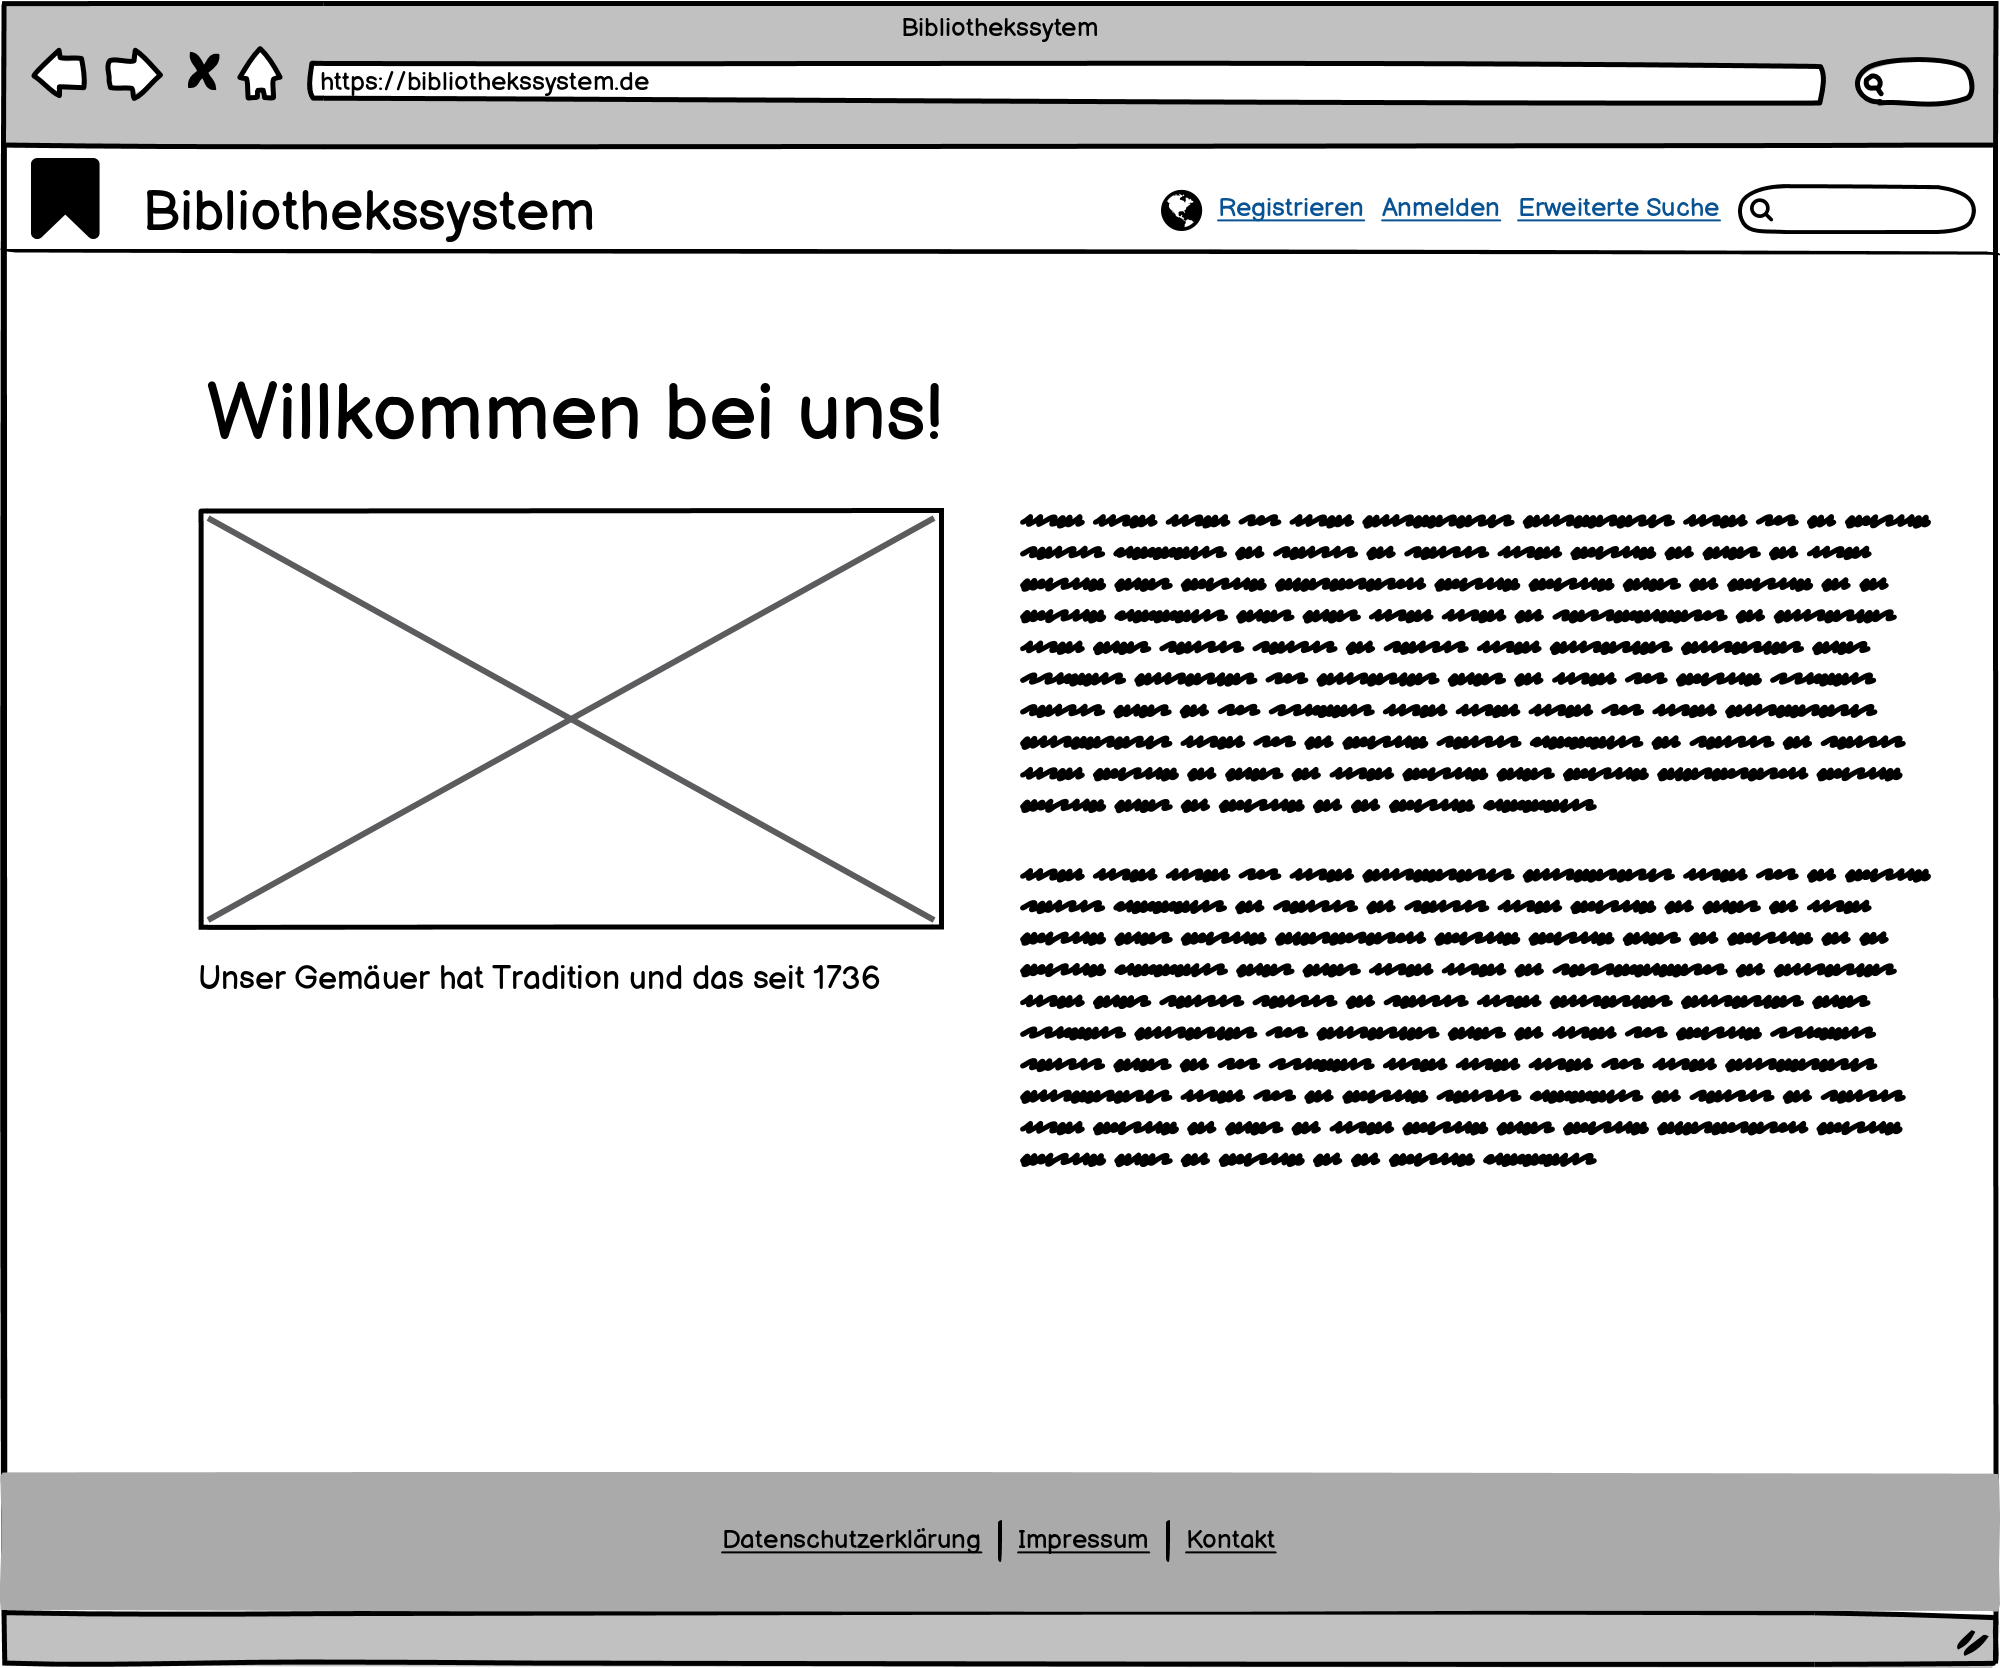
\includegraphics[width = 40em]{Startseite}
    \caption{Skizzierung der Startseite}
    \label{startseite}
\end{figure}

\begin{figure}[h]
    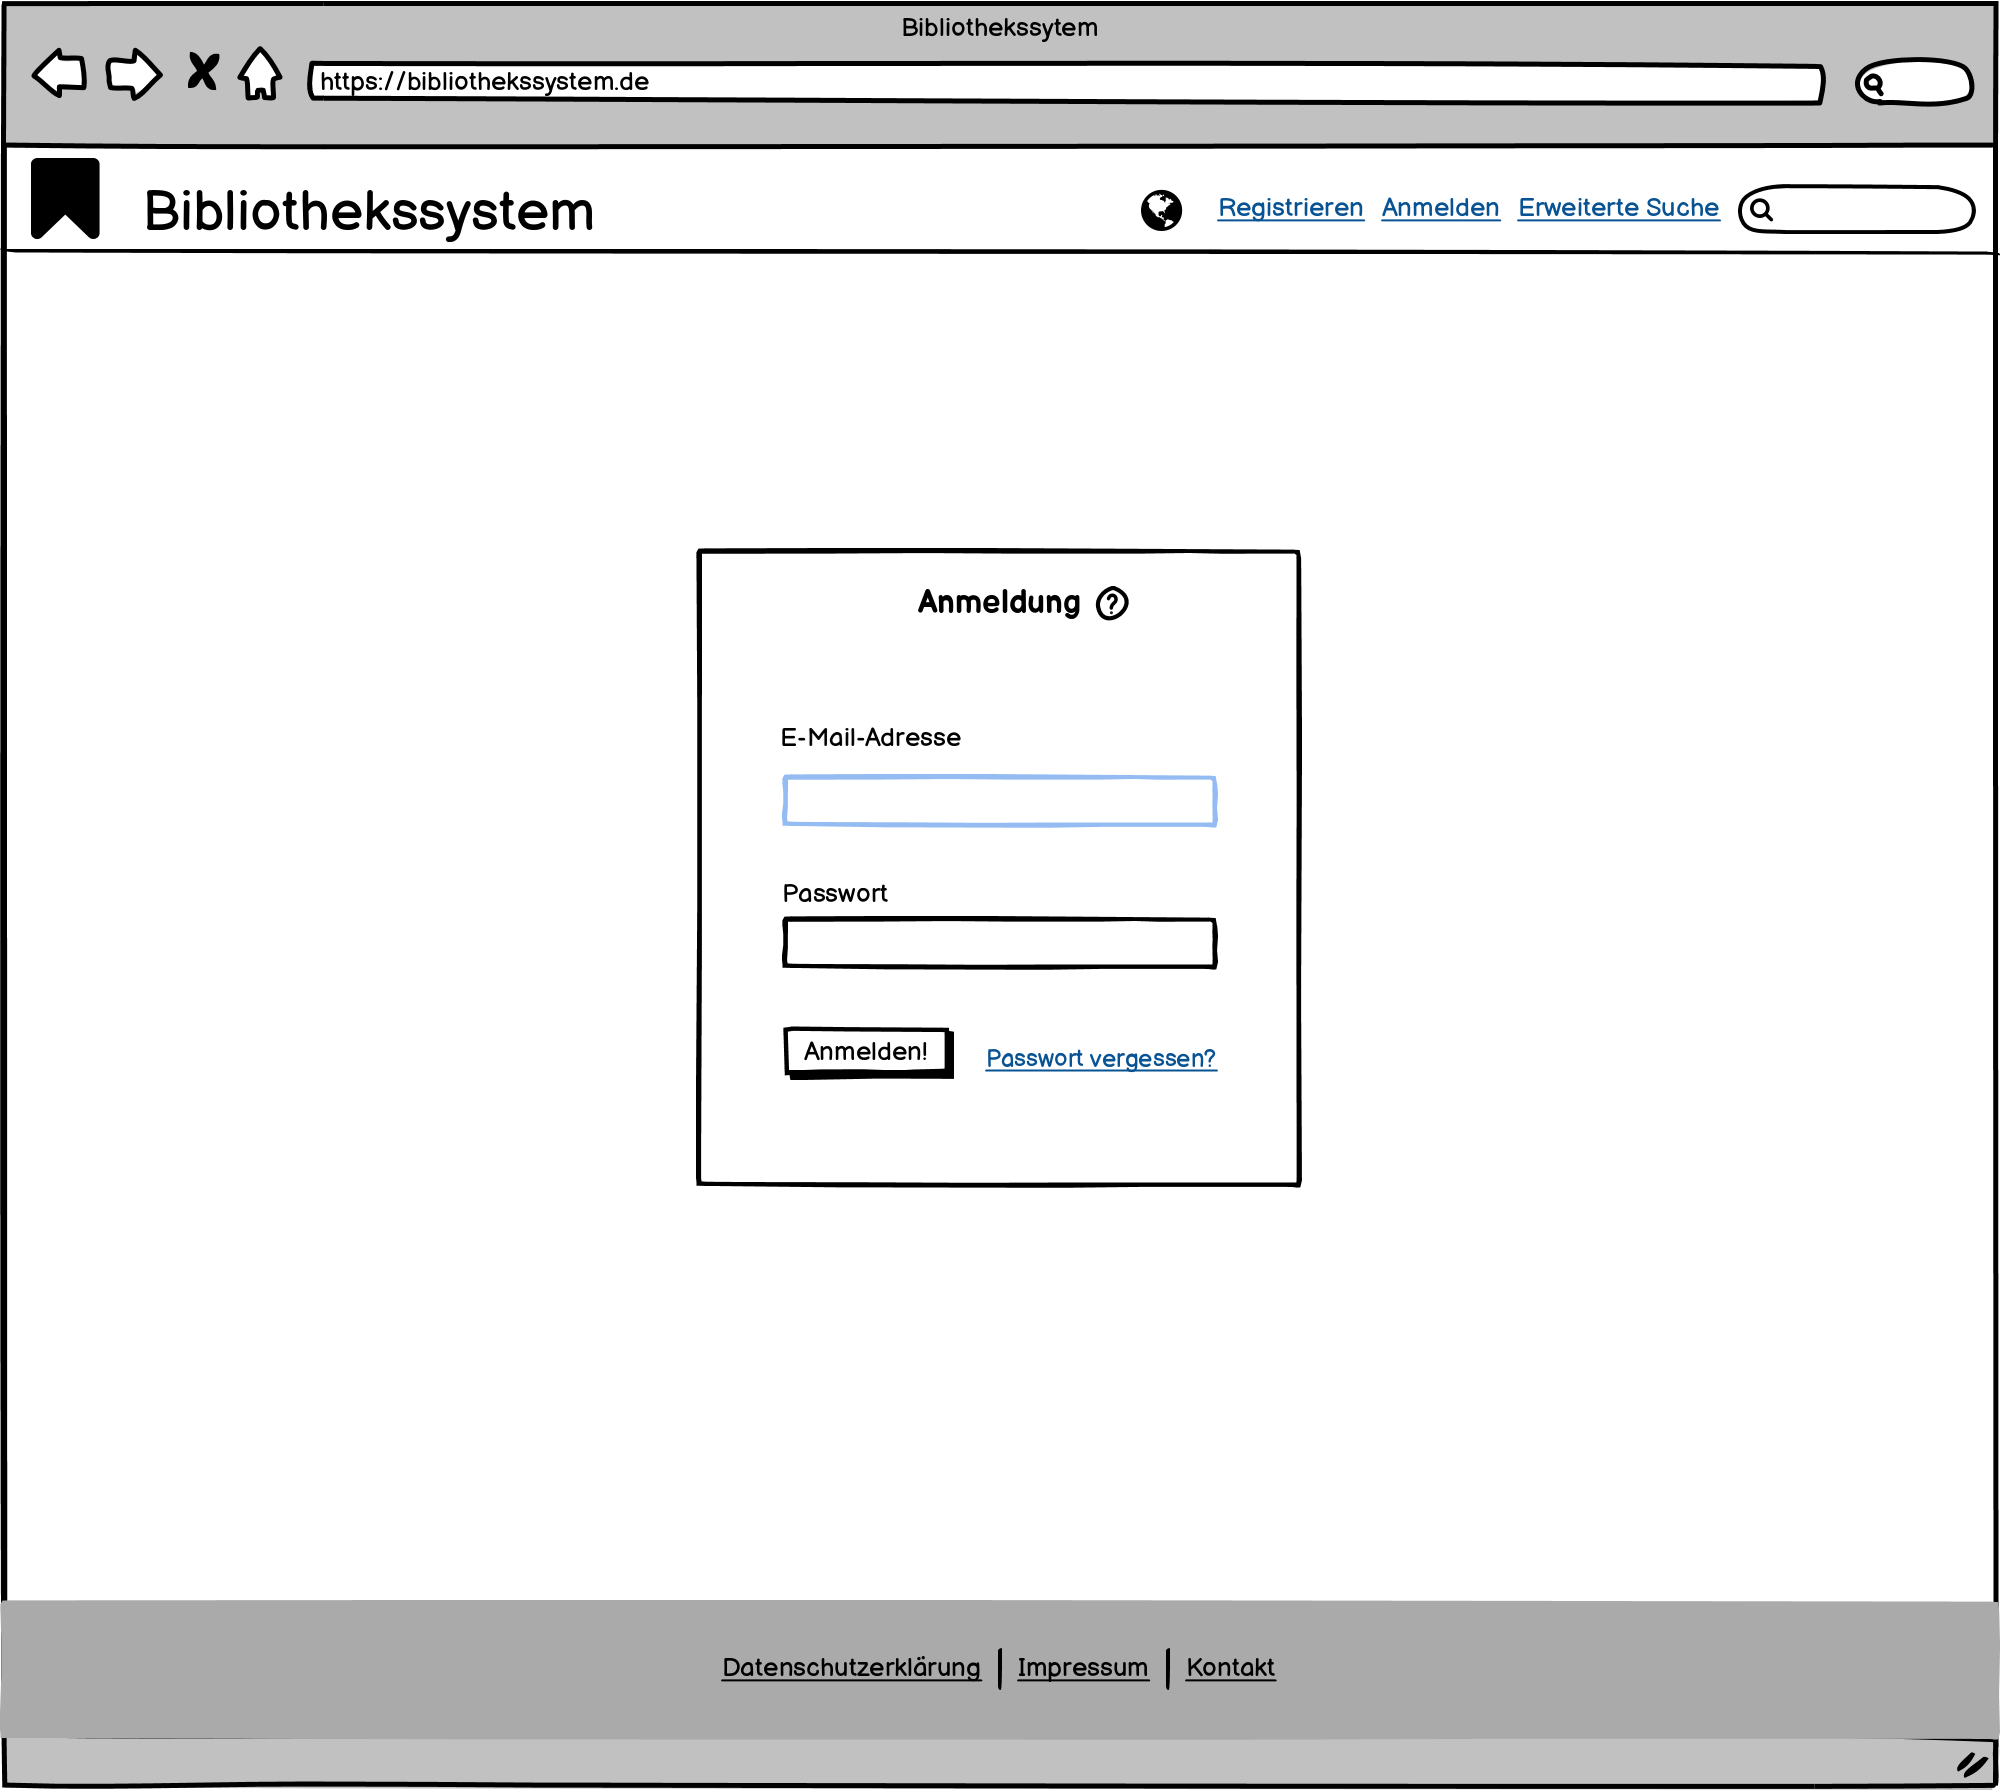
\includegraphics[width = 40em]{Anmeldemaske}
    \caption{Skizzierung der Anmeldemaske}
    \label{anmeldemaske}
\end{figure}

\begin{figure}[h]
    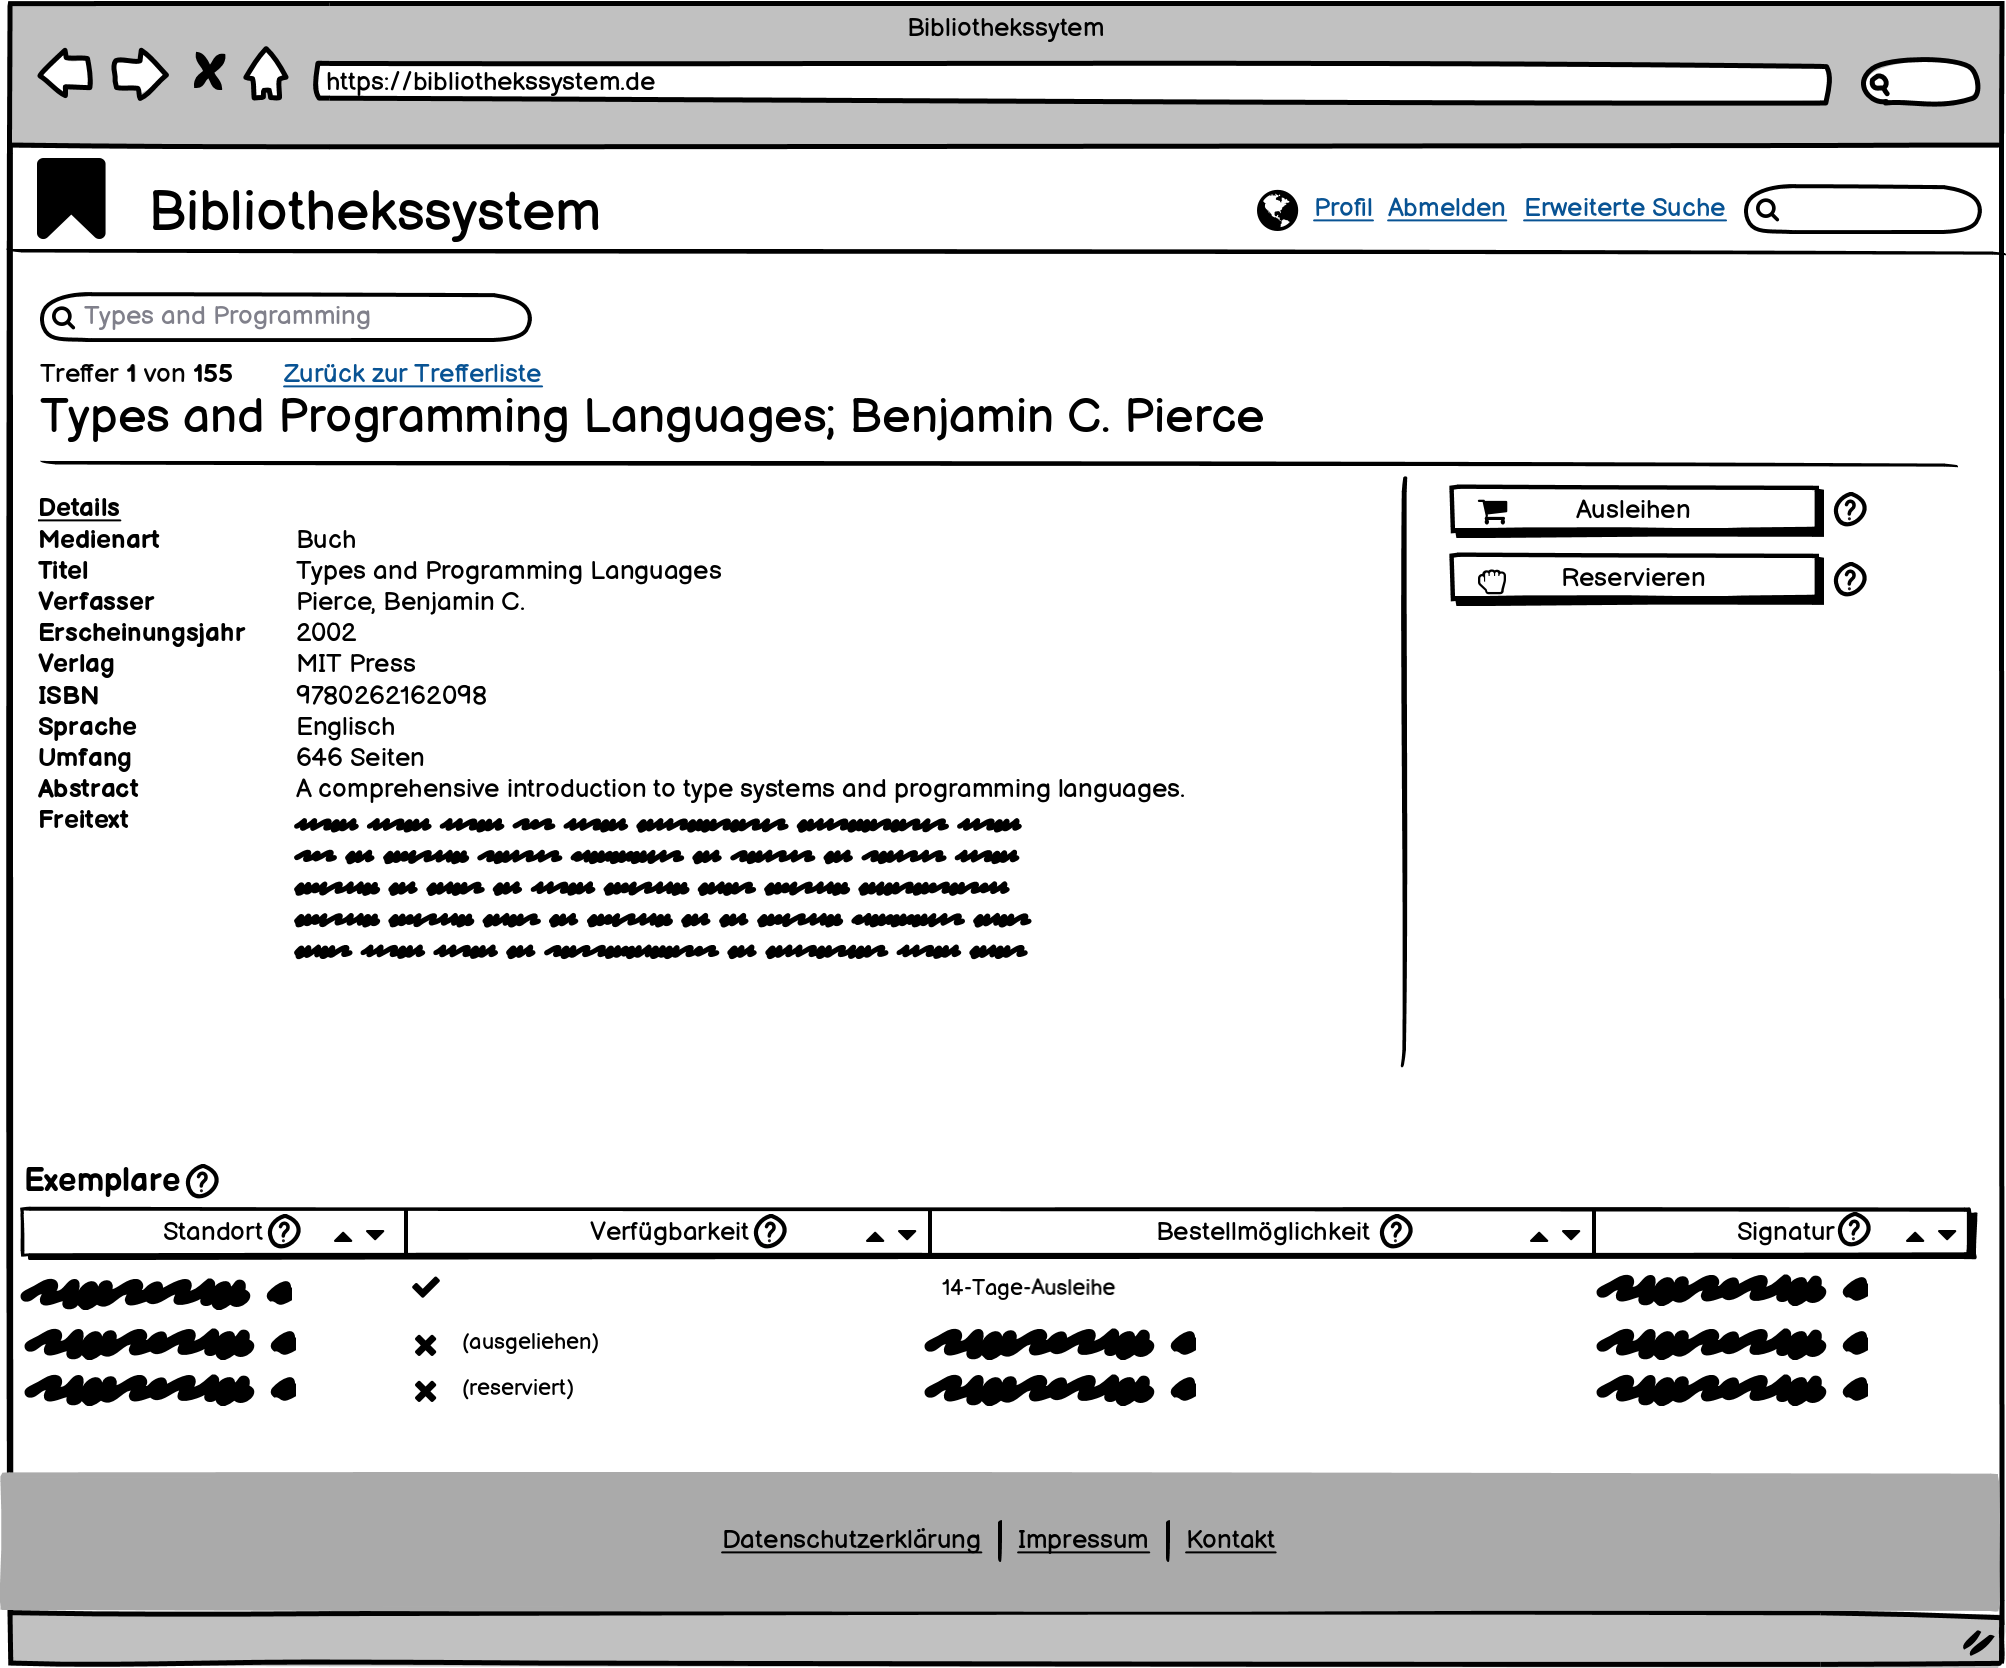
\includegraphics[width = 40em]{Mediumsseite}
    \caption{Skizzierung der Mediumsseite aus Sicht eines nicht privilegierten Nutzers}
    \label{mediumsseite_angemeldet}
\end{figure}

\begin{figure}[h]
    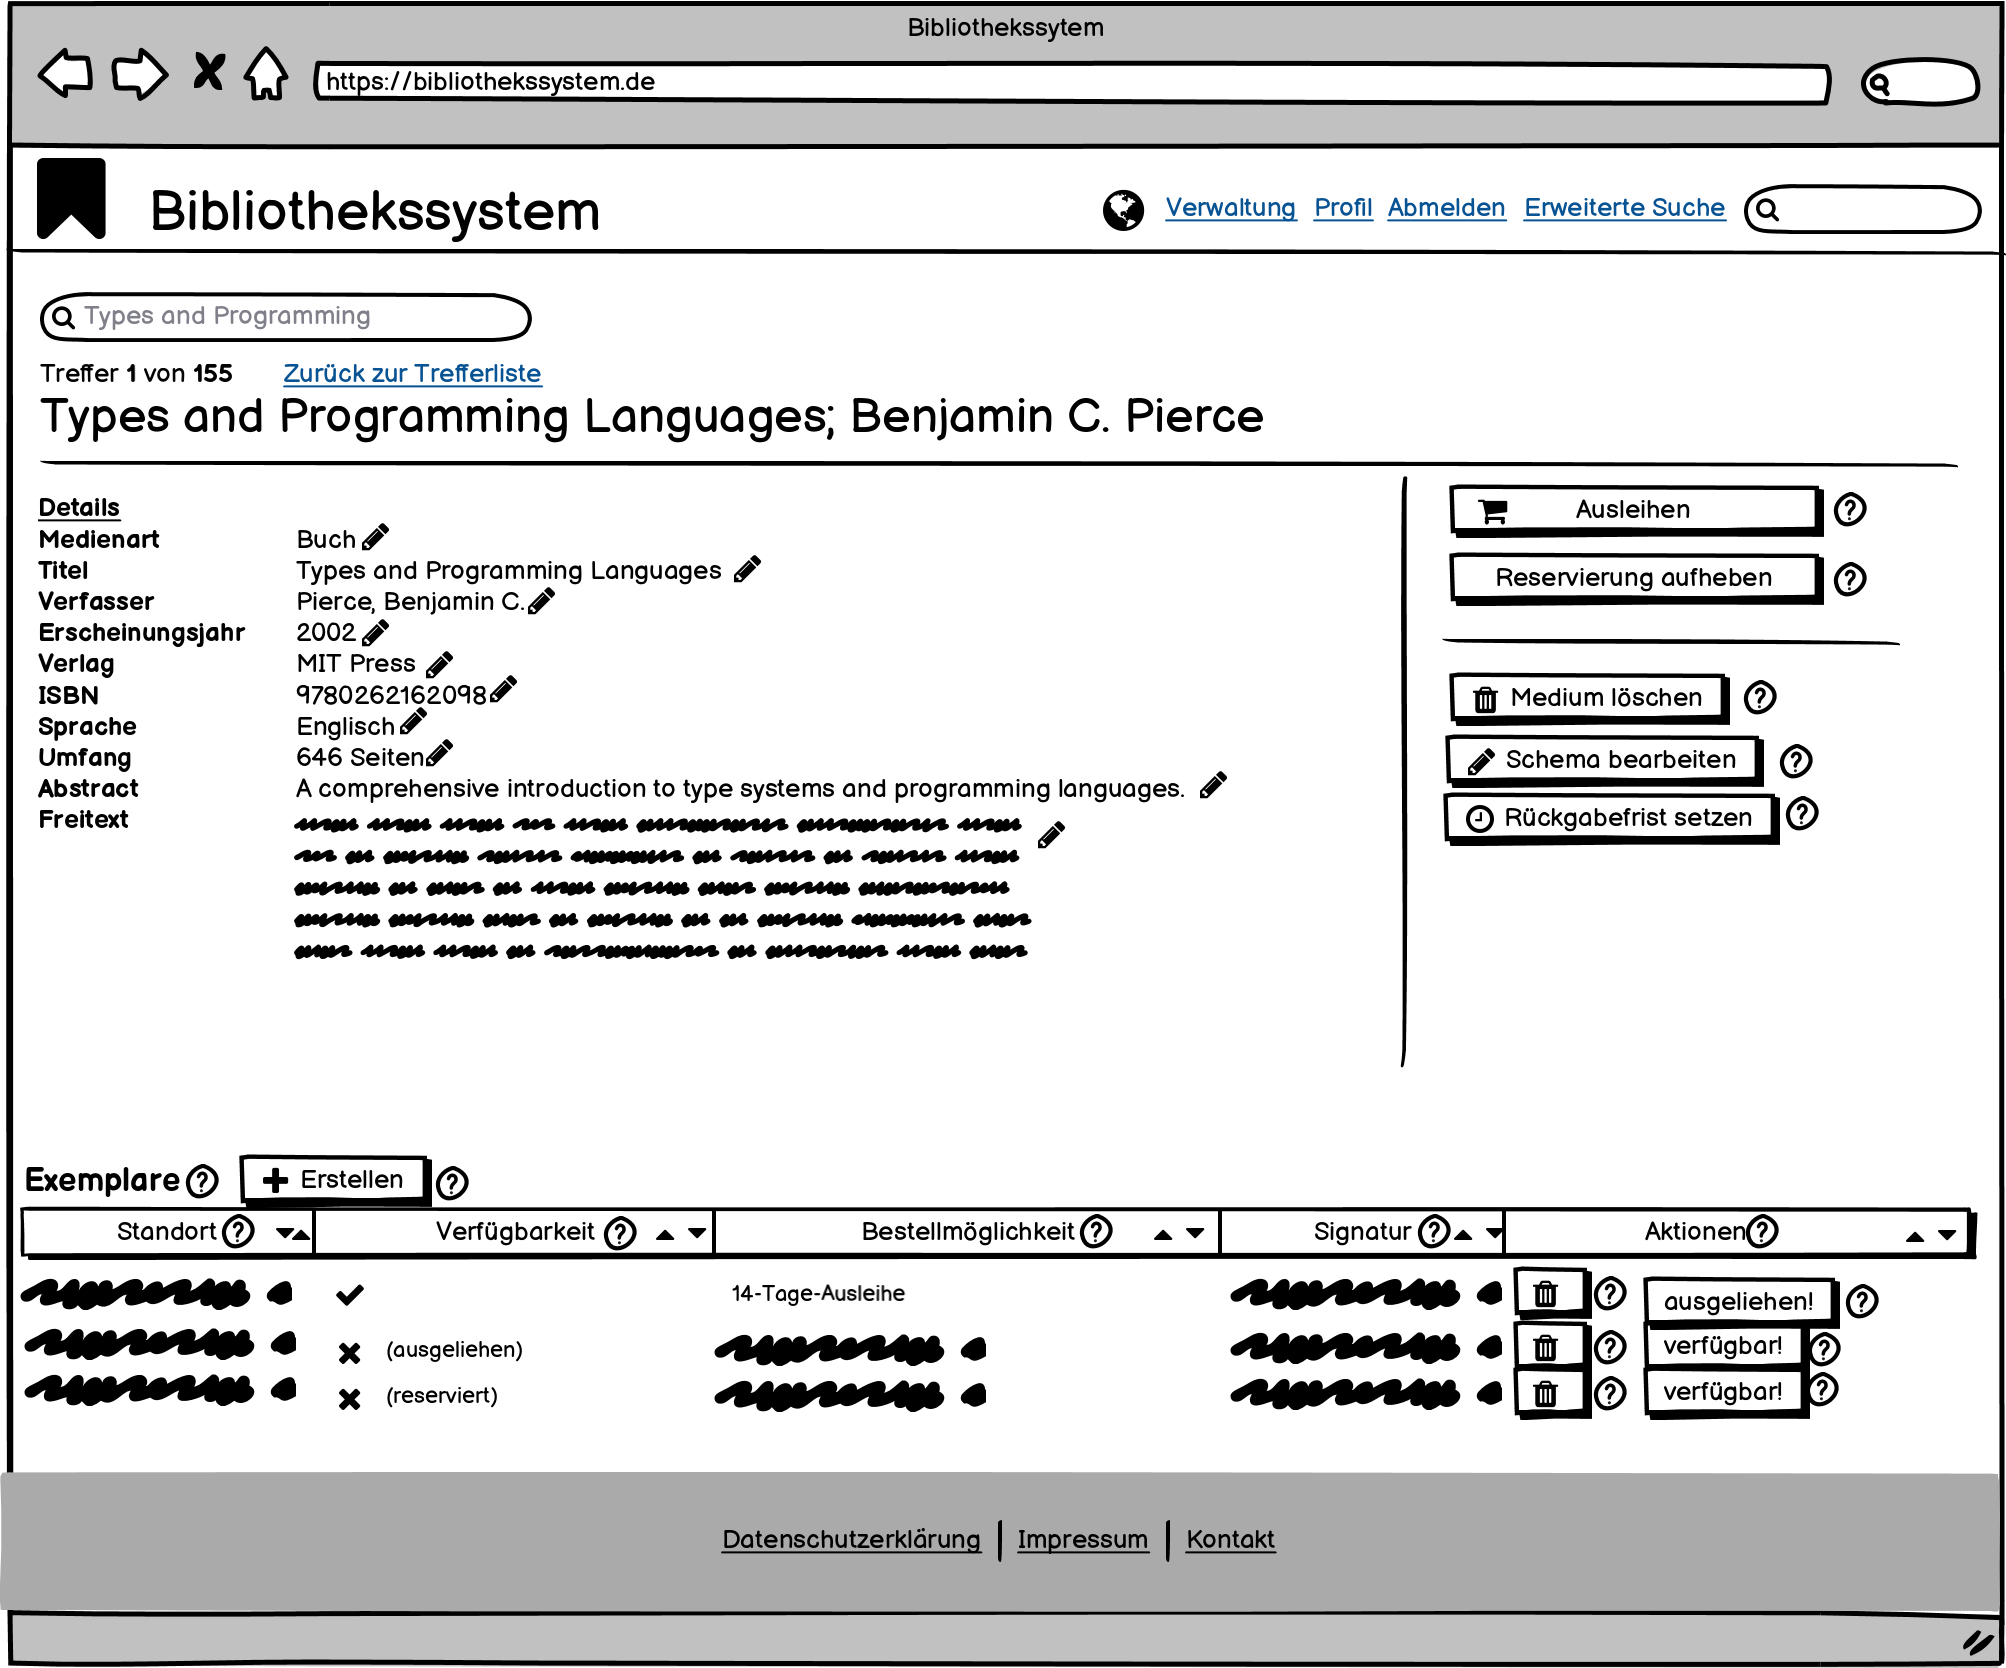
\includegraphics[width = 40em]{Mediumsseite_Admin}
    \caption{Skizzierung der Mediumsseite aus Sicht eines Administrators}
    \label{mediumsseite_admin}
\end{figure}

\newpage
\newgeometry{left=0.1cm,right=0.1cm,top=0.1cm,bottom=0.1cm}

\begin{figure}[h]
    \centering
    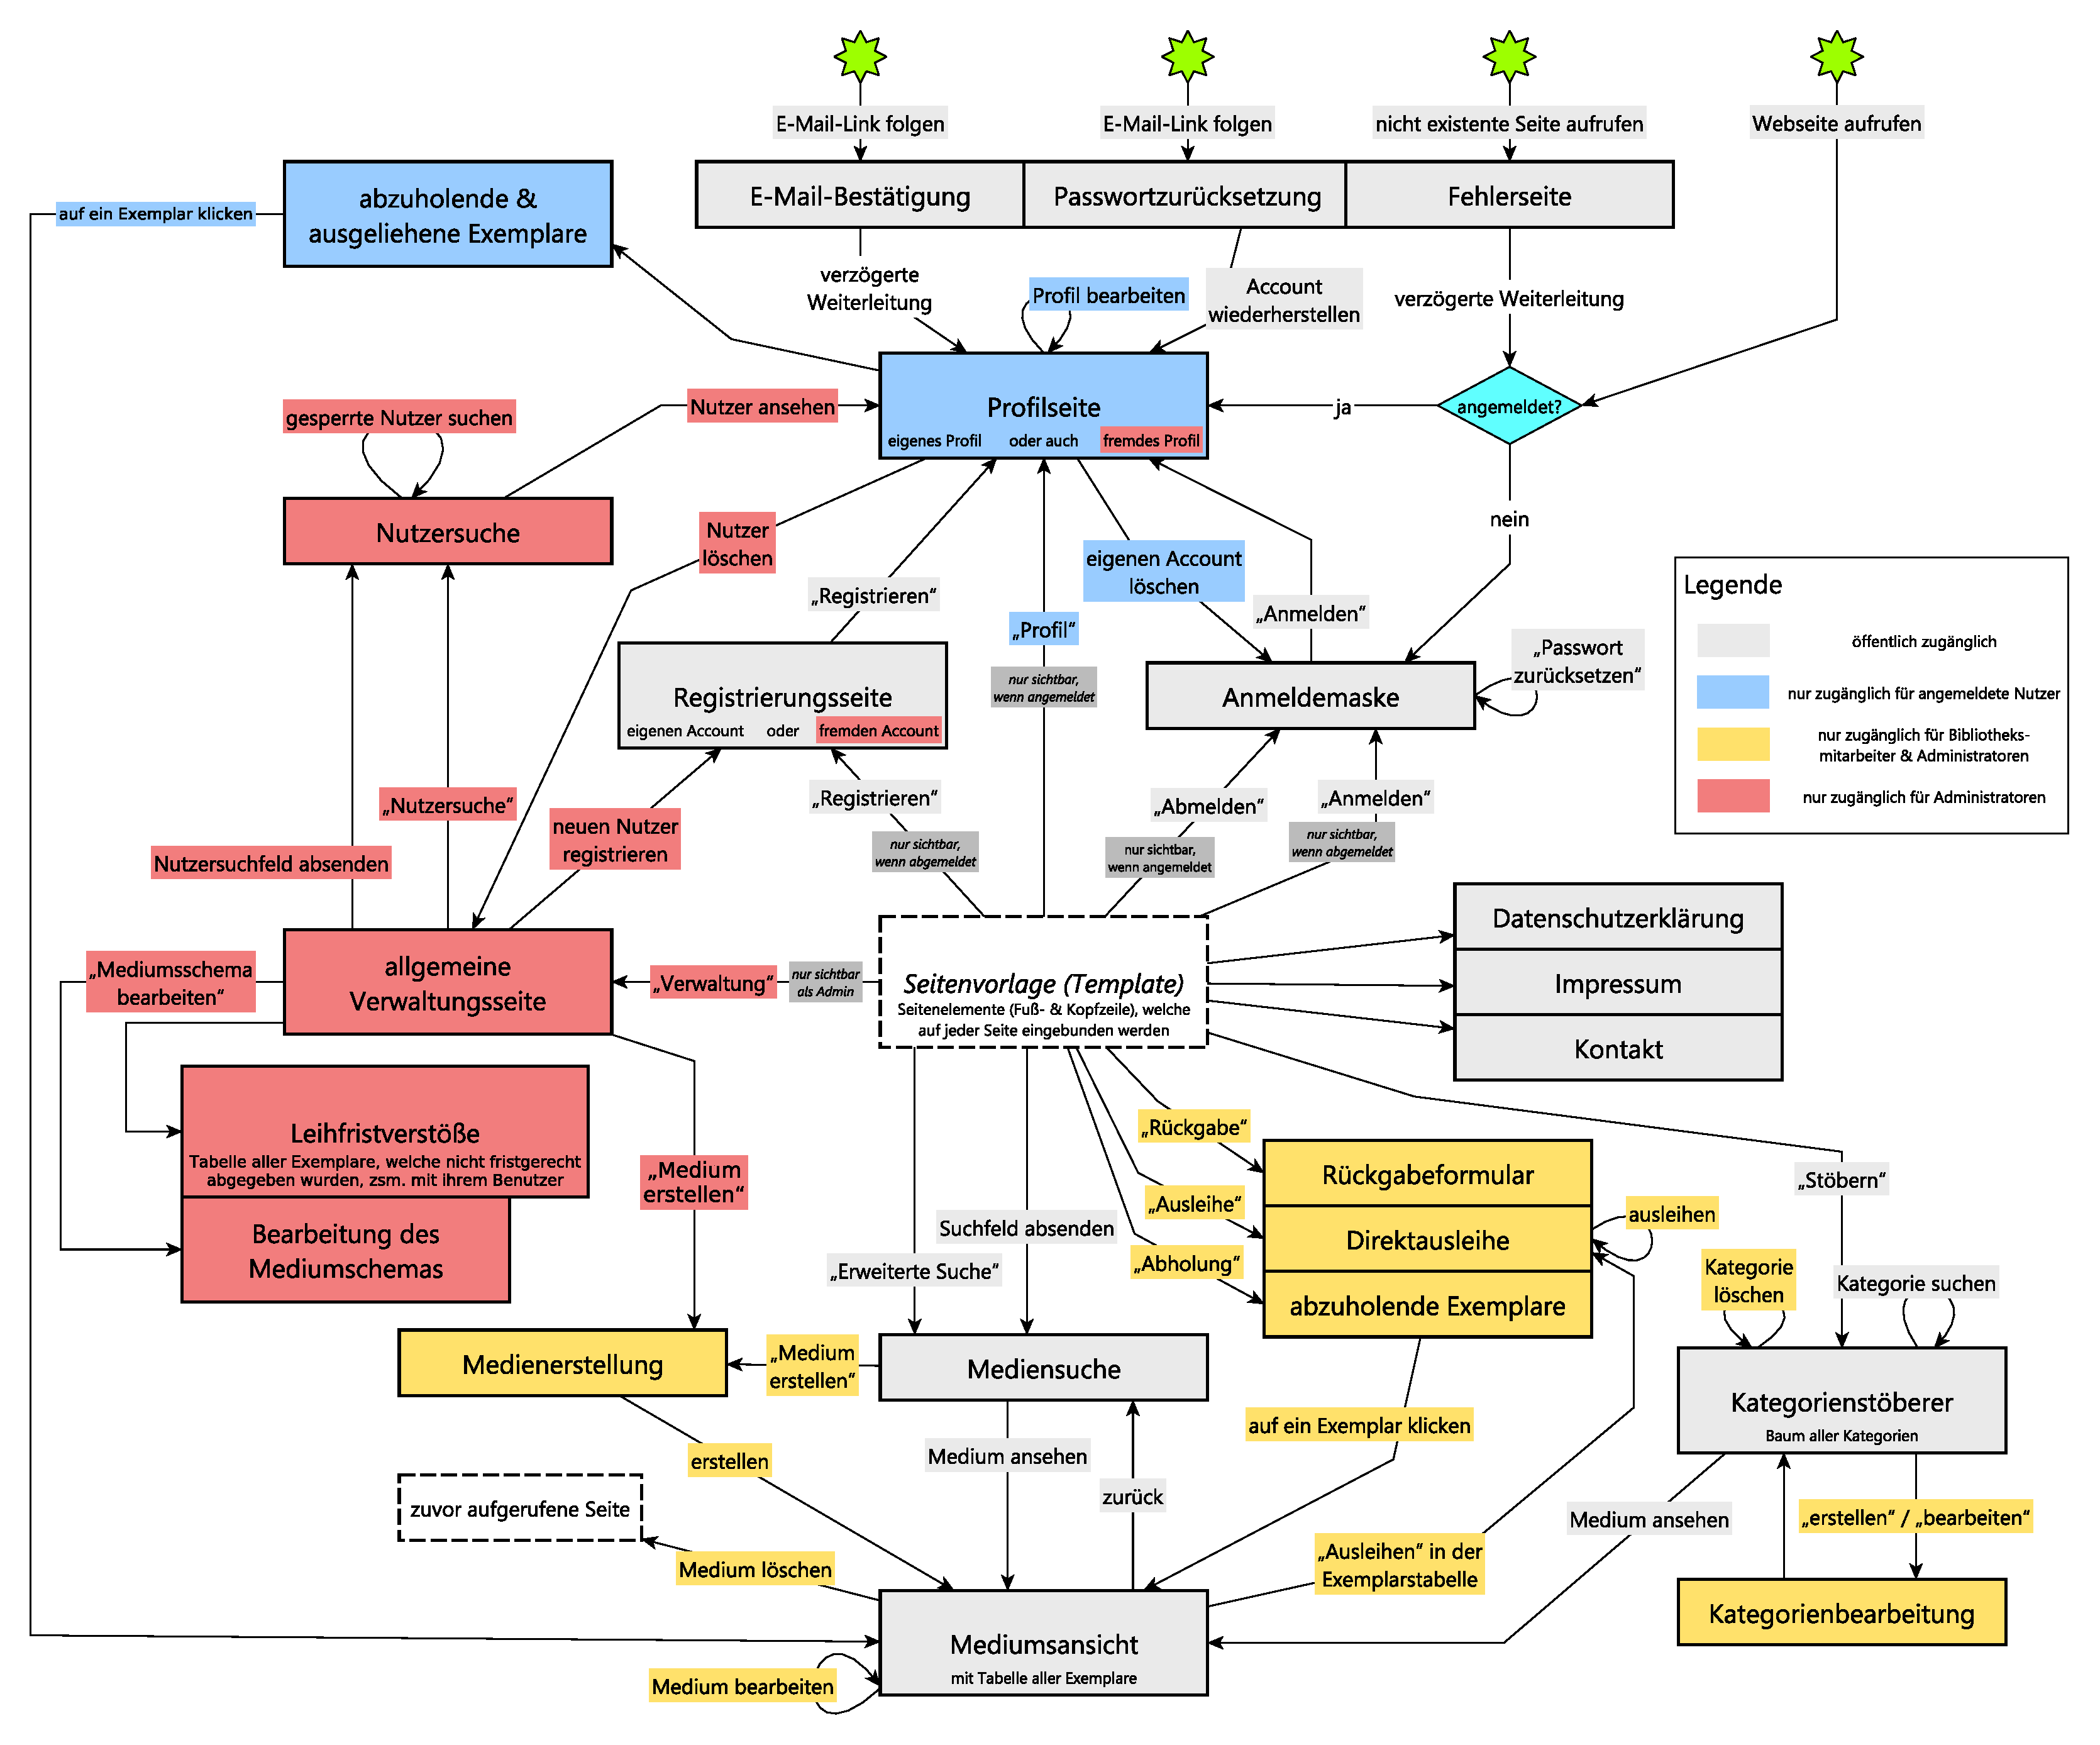
\includegraphics[angle = 270, width = 40em]{site_map}
    \caption{Die Inhaltsübersicht der Webseite (engl. \textit{site map})}
    \label{site_map}
\end{figure}

\restoregeometry

\section{Qualitätsanforderungen} %-------------------------------------------------------------------------------------------------
\sectionauthor{Mohamad Najjar}

	Die folgende Tabelle zeigt die Priorität, die jeder Qualitätsanforderung zugewiesen wird.
	
\begin{center}
\begin{tabular}{ |l||c|c|c|c| } 
 \hline
  & sehr wichtig & wichtig & weniger wichtig & unwichtig \\
 \hline\hline
 Benutzerfreundlichkeit & X & & & \\
 \hline
 Funktionalität & X & & & \\ 
 \hline
 Korrektheit & X & & & \\
 \hline
 Robustheit & & X & & \\
 \hline
 Vertrauenswürdigkeit & & X & & \\
 \hline
 Effizienz & & X & & \\
 \hline
 Änderbarkeit & & X & & \\
 \hline
 Portierbarkeit & &   & X & \\

 \hline
\end{tabular}
\end{center}
\begin{itemize}
\item Da  unser System einfach und intuitiv zu bedienen sein soll und die häufigsten Funktionen sollten
 zugänglich sein, wird sehr wichtig  auf die Benutzerfreundlichkeit und Funktionalität gesetzt.
\item Aus dem Grund, dass sensible Daten zu jedem Zeitpunkt nur für Berechtigte zugänglich sind, wird auf  wichtig gesetzt.
\item Um nachträgliche Änderungen und Erweiterungen einfach vornehmen zu können, 
sollte das System in gewissen Grenzen flexibel genug sein.
\item Um Manipulationen mit bekannten Angriffsmethoden zu verhindern, werden bestimmte Maßnahmen getroffen.
\end{itemize}
\section{Blackbox-Tests} %-------------------------------------------------------------------------------------------------
\sectionauthor{Sergei Pravdin}
Das Bibliothekssystem ist erfolgreich eingesetzt und so eingestellt, dass eine Registrierung für alle E-Mail-Domänen möglich ist. Das System hat einen Administrator namens Max Mustermann mit der E-Mail-Adresse 'admin.sep2021.test@gmail.com', der Anschrift 'Innstraße 33, 94032 Passau, Deutschland' und dem Kennwort 'xlA24!bGhm'. Außerdem verfügt das Impressum in der Anschrift die Innstraße. \vspace{0.5em}

Die im Folgenden beschriebenen Testfälle bauen aufeinander auf. Das bedeutet, dass der Zustand des Systems für den folgenden Testfall übernommen wird.
\subsection{Testfälle}
\specification{T}{010}{Die Webseite des Systems wird aufgerufen. Der Administrator gibt die E-Mail-Adresse 'admin.sep2021.test@gmail.com' und das Kennwort 'xlA24!bGhm' in die Anmeldungsfelder 'E-Mail-Adresse' und 'Passwort' ein und klickt auf 'Anmelden'. Die Anmeldung ist erfolgreich und die Profilseite mit dem Nachnamen 'Mustermann' wird gezeigt. ­­­­­ (\hyperlink{spec:F:100}{/F100/}) }
\specification{T}{011}{Der Administrator klickt auf 'Allgemeine Verwaltungsseite' und dann auf 'Mediumsschema bearbeiten'. Er gibt '00:00:01' (1 Minute) im Feld Ausleihdauer ein und klickt auf 'Speichern'. Die Seite 'Bearbeitung des Mediumsschemas' wird erneut geladen und die Ausleihdauer '00:00:01' ist sichtbar. (\hyperlink{spec:F:240}{/F240/}) (\hyperlink{spec:F:270}{/F270/})}
\specification{T}{020}{Der Administrator klickt auf 'Verwaltung' und im Anschluss auf 'Neuen Nutzer registrieren'. Die Registrierungsseite wird geladen und der Administrator gibt im Registrierungsformular als E-Mail-Adresse, Kennwort, Vorname, Name, Straße, Hausnummer, PLZ, Stadt, Land folgende Daten an:  'mitarbeiter.sep2021test@gmail.com', 'sijAs13!!A', 'Tom', 'Mustermann', 'Instraße', '33', '94032', 'Passau', 'Deutschland'. Anschließend klickt er auf 'Bearbeiten', definiert die Rolle des Profiles als 'Mitarbeiter' und klickt auf 'Speichern'. Danach klickt er auf 'Registrieren', 'Abmelden' und gibt die E-Mail-Adresse 'mitarbeiter.sep2021test@gmail.com' sowie das Kennwort 'sijAs13!!A' in die Anmeldungsfelder 'E-Mail-Adresse' und 'Passwort' ein. Er klickt auf 'Anmelden'. Die Anmeldung ist erfolgreich und die Profilseite mit dem Nachnamen 'Mustermann' und mit dem Vornamen 'Tom' wird gezeigt. (\hyperlink{spec:F:110}{/F110/}) (\hyperlink{spec:F:30}{/F30}) }
\specification{T}{030}{Der Mitarbeiter klickt auf 'Profil bearbeiten', setzt 'Müller' als Nachname und klickt auf 'Speichern'. Die Profilseite wird wiedergeladen und der Nachname 'Müller' ist sichtbar. ­­­­­ (\hyperlink{spec:F:120}{/F120/}) }
\specification{T}{040}{Der Mitarbeiter klickt auf 'Erweiterte Suche', im nächsten Schritt auf 'Medium erstellen', gibt im Formular '17RE', 'Buch', 'Programmieren lernen', '1.0', 'Mustermann', '2020', 'Springer' als 'Index', 'Typ', 'Titel', 'Version', 'Autoren', 'Erscheinungsdatum' und 'Herausgeber' ein und klickt auf 'Erstellen'. Die Seite des Mediums wird geladen und der Index '17RE' ist sichtbar. ­­­­­ (\hyperlink{spec:F:380}{/F380/}) (\hyperlink{spec:F:400}{/F400/})}
\specification{T}{050}{Der Mitarbeiter befindet sich auf der Seite des Mediums 'Programmieren lernen' und klickt 'Medium bearbeiten'. In der Tabelle aller Exemplare gibt er die Signatur '17RE (+1)' ein und klickt im Anschluss auf 'Speichern'. Die Seite wird erneut geladen und die Signatur 17RE (+1)' ist sichtbar. ­­­­­ (\hyperlink{spec:F:420}{/F420/}) (\hyperlink{spec:F:190}{/F190/})}
\specification{T}{060}{Der Mitarbeiter klickt auf 'Stöbern', dann auf 'Kategorie erstellen' und gibt im Formular 'Informatik' und 'Alle Medien zu Informatik' als 'Name', und 'Beschreibung' ein. Anschließend klickt er auf 'Speichern'. Der Kategorienstöberer wird geladen und die Kategorie 'Informatik' ist sichtbar. ­­­­­ (\hyperlink{spec:F:360}{/F360/})}
\specification{T}{070}{Der Mitarbeiter gibt im Suchfeld 'Programmieren lernen' ein und sendet den Suchauftrag ab. Die Seite 'Mediensuche' wird geladen und das Medium mit Titel 'Programmieren lernen' ist sichtbar. Im nächsten Schritt klickt der Mitarbeiter auf dieses Medium, die Seite des Mediums wird geladen. Danach klickt der Mitarbeiter auf 'Medium bearbeiten', definiert im Attributsformular die Kategorie 'Informatik­­­­­' und klickt dann auf 'Speichern'. Er klickt nun auf 'Stöbern', der Kategorienstöberer wird geladen und das Medium ist mit dem Titel 'Programmieren lernen' unter der Kategorie 'Informatik' im Baum aller Kategorien sichtbar.  (\hyperlink{spec:F:160}{/F160/}) (\hyperlink{spec:F:170}{/F170/})}
\specification{T}{080}{Der Mitarbeiter klickt auf 'Abmelden' und im nächsten Schritt auf 'Impressum'. Die Seite mit dem Impressum wird geladen und 'Innstraße' wird in der Anschrift auf der Seite sichtbar. ­­­­­ (\hyperlink{spec:F:210}{/F210/})}
\specification{T}{090}{Der Nutzer gibt im Suchfeld 'Informatik Springer' ein und sendet die Suchanfrage ab. Die Seite zur Mediensuche wird geladen und das Medium mit dem Titel 'Programmieren lernen' ist sichtbar. ­­­­­ (\hyperlink{spec:F:180}{/F180/})}
\specification{T}{100}{Der Nutzer klickt auf 'Registrierung'. Die Registrierungsseite wird geladen und der Nutzer gibt im Registrierungsformular als E-Mail-Adresse, Kennwort, Vorname, Name, Straße, Hausnummer, PLZ, Stadt, Land folgende Daten ein: 'nutzer.sep2021test@gmail.com', 'sdfHs4!a', 'Bob', 'Mustermann', 'Innstraße', '40', '94032', 'Passau', 'Deutschland'. Danach klickt er auf 'Registrieren'. Anschließend bestätigt er seine E-Mail-Adresse durch den Verifizierungslink. Die Anmeldung ist erfolgreich und als Ergebnis wird die Profilseite mit dem Vornamen 'Bob' und der E-Mail-Adresse 'nutzer.sep2021test@gmail.com' angezeigt.  ­­­­­ (\hyperlink{spec:F:90}{/F90/})}
\specification{T}{110}{Der Nutzer klickt auf 'Abmeldung', gibt als E-Mail-Adresse \linebreak  'nutzer.sep2021test@gmail.com' ein und klickt auf 'Passwort vergessen'. Anschließend \linebreak  bestätigt er seine E-Mail-Verifizierung durch den Verifizierungslink. Die Wiederherstellungsseite wird geladen und der Nutzer gibt im Wiederherstellungsformular zwei Mal das neue Kennwort 'djnASdd1d!' ein. Anschließend klickt er auf 'Speichern'; es wird eine Profilseite als Ergebnis geladen. Auf der Seite ist der Vorname 'Bob' sichtbar.­(\hyperlink{spec:F:101}{/F101/})}
\specification{T}{120}{Der Nutzer klickt auf 'Stöbern' und auf das Medium 'Programmieren lernen'. Anschließend klickt er auf 'Buchen'. Die Mediumseite wird wiedergeladen und der Status des Exemplars 'Gebucht' ist sichtbar. ­­ (\hyperlink{spec:F:330}{/F330/})}
\specification{T}{130}{Der Nutzer klickt auf 'Abmelden' und wird auf die Anmeldungsseite weitergeleitet. Er gibt dort die E-Mail-Adresse 'mitarbeiter.sep2021test@gmail.com' und das Kennwort 'sijAs13!!A' in die Formularfelder 'E-Mail-Adresse' und 'Passwort' ein und klickt auf 'Anmelden'. Nach erfolgreicher Anmeldung navigiert er durch einen Klick auf 'Abholung' zur Listenansicht der abzuholenden Exemplare. Die Seite wird geladen und der Mitarbeiter klickt auf 'abgeholt' bei dem Listeneintrag mit der Signatur '17RE (+1)'. Die Seite wird erneut geladen und der Eintrag mit der Signatur '17RE (+1)' ist verschwunden.(\hyperlink{spec:F:300}{/F300/})\hyperlink{spec:F:310}{/F310/}) }
\specification{T}{140}{Nach einer Minute klickt der Mitarbeiter auf 'Rückgabe' und die Seite mit dem Rückgabeformular wird geladen. Der Mitarbeiter gibt die Signatur '17RE (+1)' und die E-Mail-Adresse \linebreak 'nutzer.sep2021test@gmail.com' in die entsprechenden Formularfelder ein und klickt anschließend auf \linebreak 'Bestätigen'. Eine entsprechende Meldung über die erfolgreiche Zurücknahme wird sichtbar. (\hyperlink{spec:F:300}{/F300/})\hyperlink{spec:F:320}{/F320/}) }
\specification{T}{150}{Der Mitarbeiter klickt auf 'Ausleihe' und gibt auf der Seite 'Direktausleihe' im Formular die Signatur '17RE (+1)' und die E-Mail-Adresse 'nutzer.sep2021test@gmail.com' ein und bestätigt seine Eingabe. Somit ist die direkte Ausleihe erfolgreich abgeschlossen und eine entsprechende Meldung auf der Seite sichtbar ist. (\hyperlink{spec:F:321}{/F321/})}
\specification{T}{160}{Der Mitarbeiter klickt auf 'Abmelden' und die Anmeldungsmaske wird geladen. Der Administrator gibt die E-Mail-Adresse 'admin.sep2021.test@gmail.com' und das Kennwort 'xlA24!bGhm' in die Anmeldungsfelder 'E-Mail-Adresse' und 'Passwort' ein und klickt auf 'Anmelden'. Nach erfolgreicher Anmeldung klickt er auf 'Verwaltung' und navigiert zur Listenansicht 'Leihfristverstöße'. Nach dem Laden der Seite ist das Exemplar mit der Signatur '17RE (+1)', sowie der Nutzeraccount mit der E-Mail 'nutzer.sep2021test@gmail.com' und die Zeitangabe der überzogenen Frist ist sichtbar.(\hyperlink{spec:F:280}{/F280/})}
\specification{T}{170}{Der Administrator klickt auf 'Verwaltung', navigiert von dort aus zur Nutzersuche und gibt nach laden der Seite 'Bob Mustermann' im Suchfeld ein. Anschließend sendet er die Suchanfrage an und die Seite 'Nutzersuche' wird geladen, auf der der Nutzer 'Mustermann' sichtbar ist.(\hyperlink{spec:F:60}{/F60/})}
\specification{T}{180}{Der Administrator klickt auf 'Verwaltung' und dann auf 'Bearbeiten'. Im Formular gibt er 'grün', 'gelb' und 'Testsystem' in die Felder 'Farbe 1' , 'Farbe 2' und 'Name der Einrichtung' ein. Schließlich klickt er auf 'Speichern'. Die 'Allgemeine Verwaltungsseite' wird erneuet geladen und die Farben 'grün' und 'gelb', sowie der Name 'Testsystem' sind auf der Seite sichtbar. (\hyperlink{spec:F:450}{/F450/}) (\hyperlink{spec:F:470}{/F470/})}
\specification{T}{190}{Der Administrator klickt auf 'Impressum' und dann auf 'Bearbeiten'. Im Formular gibt er 'Germany' im Feld 'Land' ein. Schließlich klickt er auf 'Speichern'. Die Seite 'Impressum' wird erneuet geladen und das Land 'Germany' auf der Seite sichtbar.(\hyperlink{spec:F:480}{/F480/})}

\section{Entwicklungsumgebung} %-------------------------------------------------------------------------------------------------
\sectionauthor{Jonas Picker}

Die Entwicklung finden auf verschiedenen Privatrechnern der Teammitglieder statt, deren Bauteile und Betriebssysteme in den folgenden Listen kurz umrissen werden, keiner der Rechner weißt sonstige Besonderheiten auf. 

\subsection{Software}

\begin{itemize}
\item \underline{\textbf{Dokumentenbearbeitung}}: 
\begin{flushleft}
LaTeX Distribution MiKTeX, Version: 21.2 \linebreak
Overleaf Online Latex Editor \linebreak
LaTeX Distribution MacTeX-2021 \linebreak
\end{flushleft}
\item \underline{\textbf{Webbrowser}}:
\begin{flushleft}
Google Chrome, Version: 88.0 \linebreak
Mozilla Firefox, Version: 85.0 \linebreak
Apple Safari, Version: 14.0.3 \linebreak
\end{flushleft}
\item \underline{\textbf{Integrierte Entwicklungsumgebungen}}: 
\begin{flushleft}
Eclipse IDE for Enterprise Java Developers, Version: 2020-12 (4.18.0) \linebreak
IntelliJ IDEA 2021.1 Ultimate Edition \linebreak
\end{flushleft}
\item \underline{\textbf{Objektorientierte Modellierung}}: 
\begin{flushleft}
IBM Rational Software Architect Designer 9.7 \linebreak
\end{flushleft}
\item \underline{\textbf{Programmiersprachen, Entwicklungs- \& Testframeworks}}: 
\begin{flushleft}
Java OpenJDK JDK 16 GA-Release\linebreak
Jakarta EE 9 \linebreak
Jakarta Server Faces 3.0 Mojarra Implementation \linebreak
CDI 3.0 with Red Hat Weld, Version: 4.0.1.Final \linebreak
Cascading Style Sheets Level 3 \linebreak
JUnit Platform, Version: 1.7.1 \linebreak
Selenium Server (Grid), Version: 3.141.59 \linebreak
\end{flushleft}
\item \underline{\textbf{Versionsmanagement}}:
\begin{flushleft}
git, Version 2.31.1 \linebreak
\end{flushleft}
\item \underline{\textbf{Betriebssysteme der Entwicklungsrechner}}:
\begin{flushleft}
MacOS Big Sur, Versionen: 11.2.3 und 11.2.1 \linebreak
Windows 10 Home 20H2 \linebreak
GNU/Linux Arch, Version: 5.11.11 \linebreak
GNU/Linux Debian, Version: 4.19.132-1 \linebreak
\end{flushleft}
\item \underline{\textbf{Graphische Prototypenbearbeitung}}:
\begin{flushleft}
Balsamiq Wireframes, Version: 4.2.4 \linebreak 
yEd Graph Editor, Version: 3.21.1 \linebreak 
\end{flushleft}
\item \underline{\textbf{Applikationsserver}}: 
\begin{flushleft}
Apache Tomcat, Version: 10.0.2 \linebreak
\end{flushleft}
\item \underline{\textbf{Datenbanktreiber und Visualisierung}}: 
\begin{flushleft}
PostgreSQL JDBC 4.2 Driver, Version: 42.2.19 \linebreak
DBeaver, Version: 21.0.2
\end{flushleft}
\item \underline{\textbf{Teamkommunikation}}: 
\begin{flushleft}
Slack \linebreak
Discord \linebreak
Skype \linebreak
Stud.IP \linebreak
\end{flushleft}
\end{itemize}

\subsection{Hardware}

\begin{itemize}
\item \underline{\textbf{Entwicklungsrechner}}: 
\begin{flushleft}
MacBook Pro, 8GB RAM, Intel Core i5 2GHz  \linebreak
HP Laptop 15-db1xxx, 16GB RAM, AMD Ryzen 5 3500U 2.1GHz \linebreak
2x MacBook Pro, 8GB RAM, Intel Core i5 2.3GHz \linebreak
Tower-PC, 16GB RAM, AMD Ryzen 5 3600XT 3.8GHz \linebreak
\end{flushleft}
\item \underline{\textbf{Referenzrechner}}:
\begin{flushleft}
CIP-Pool Computer 'schratz', Uni Passau, 15.6GB RAM, Intel Core i7-4790 3.60GHz CPU, Intel I217-LM Ethernet Controller \linebreak
Spezifikation der virtualisierten Datenbank (siehe Entwicklungsschnittstellen) bezieht sich auf die Referenzhardware von 'schratz' und besitzt eine geschätze Übertragungsrate von ca. 1GB/s ins Internet. Die Datenbank unterstützt das Verschlüsselungsprotokoll TLS mit einem Zertifikat. \linebreak
\end{flushleft}
\end{itemize}

\subsection{Entwicklungsschnittstellen}

\begin{itemize}
\item \begin{flushleft} Netzwerk- und Internetverbindung \end{flushleft} 
\item \begin{flushleft} Virtuelle private Netwerkanbindung mit OpenVPN, Version 2.5.1 \end{flushleft} 
\item \begin{flushleft} Git-verwaltetes Repository der Uni Passau, Website: https://git.fim.uni-passau.de/ \end{flushleft} 
\item \begin{flushleft} Virtualisierte Datenbank der Uni Passau, Hostname: bueno.fim.uni-passau.de \end{flushleft}
\end{itemize}

\section{Glossar} %-------------------------------------------------------------------------------------------------
\sectionauthor{Jonas Picker}

\begin{itemize}\item OPAC (5.1)
\begin{flushleft}
Online public access catalog, darunter versteht man den über das Internet zugänglichen Bibliothekskatalog, mit dem der Bestand an Publikationen recherchiert werden kann.
\end{flushleft}
\item Webbrowser (Einleitung)
\begin{flushleft}
Spezielle Computerprogramme zum Anzeigen von Webseiten im World Wide Web. Bekannte Beispiele sind: Google Chrome, Apple Safare, Mozilla Firefox.
\end{flushleft}
\item Adressraum (2.1)
\begin{flushleft}
Die in der Kopfzeile des Browsers angezeigte Adresse unter der die Anwendung erreichbar seien soll, Unterabschnitte des Systems bauen auf diesem getzten Wert auf.
\end{flushleft}
\item Look \& Feel (2.1)
\begin{flushleft}
Die Umschreibung der Kombination aus Farbauswahl und Form sowie Größe und Position der Elemente einer Webseite.
\end{flushleft}
\item HTML (4.1)
\begin{flushleft}
Die Hypertext Markup Language ist eine textbasierte Auszeichnungssprache, die als Dokumentenstandart eine Grundlage des World Wide Webs bildet.
\end{flushleft}
\item CSS (4.1)
\begin{flushleft}
Cascading Style Sheets ist eine weitere Auszeichnungssprache mit der unter anderem die Darstellung, Form, Farben und Positionen der Elemente einer Webseite verändert werden kann.
\end{flushleft}
\item JavaScript (4.1)
\begin{flushleft}
Ist eine Skriptsprache, die hauptsächlich dazu verwendet wird, die Logik hinter interaktiven Elementen einer Webseite zu formulieren.
\end{flushleft}
\item Laufzeitumgebung (4.1)
\begin{flushleft}
Hierunter versteht man die für eine Programmiersprache zur Ausführungszeit verfügbaren und festgelegten Voraussetzungen.
\end{flushleft}
\item SSL/TLS (4.1)
\begin{flushleft}
Das Secure Socket Layer- bzw. Transport Layer Security-Protokoll bietet die Möglichkeit zur sicheren Datenübertragung über das Internet, hierzu ist ein kryptographisches Schlüsselzertifikat nötig.
\end{flushleft}
\item SMTP (4.1)
\begin{flushleft}
Das Simple Mail Transfer Protocol wird zum Weiterleiten und Verschicken von E-Mails verwendet.
\end{flushleft}
\item VPN (4.2)
\begin{flushleft}
Virtual Private Network meint hier den verschlüsselten Fernzugriff auf Ressourcen in einem fremden lokalen Netzwerk über einen 'Tunnel' durch das Internet.
\end{flushleft}
\item ID (6.)
\begin{flushleft}
Dies ist die Abkürzung für einen Identifikator, normalerweiße eine für den zu identifizierenden einzigartige Nummer ohne weiteren Informationsgehalt.
\end{flushleft}
\item UTF-8 (7.1)
\begin{flushleft}
Das 8-bit Unicode Transformation Format wird zur Kodierung von nahezu allen weltweit verwendeten Zahlen, Schriftzeichen und sonstigen schriftlichen Elementen verwendet.
\end{flushleft}
\item Paginierung (7.1)
\begin{flushleft}
Hierunter verstehen wir die Aufteilung von abgefrageten Listen in kleinere Abschnitte, um die Darstellung zu erleichtern und lange Ladezeiten bei großen Ergebnissen zu vermeiden.
\end{flushleft}
\item Regex-Ausdruck (5.4.1)
\begin{flushleft}
Dies bezeichnet einen regulären Ausdruck, der eine Sprache von Wörtern definiert. Eine solche reguläre Sprache hat u.a. die Eigenschaft, dass es sich berechnen lässt, ob ein gegebenes Wort in dieser Sprache liegt.
In den meisten objekt-orientierten Sprachen sind solche Ausdrücke und Überprüfungen unterstützt.
\end{flushleft}
\end{itemize}

\end{document}
